\documentclass[a4paper]{report} % estilo do documento
\usepackage[utf8]{inputenc}
\usepackage[portuges]{babel} % para selecionar o idioma português 

\usepackage{graphicx} % para importar imagens

\usepackage{array} %% necessário para a construção das tabelas

\usepackage{url} % para colocar links na bibliografia

\usepackage{fancyhdr} % para personalizar o cabeçalho e o rodapé do texto

\usepackage{underscore} % para considerar as palavras com underscore sem ter que usar tag adicional

\usepackage{makeidx} % para gerar indice automático

\begin{document}

\begin{figure}[t]
    
    \centering
    \flushleft\includegraphics[scale = 0.2]{Imagens/um.png}

\end{figure}

\title {\huge Relatório do "Micro Machines"}
\author{Grupo 13
\\
João Sampaio e José Ferreira}

\date{31 de Dezembro de 2017}

\begin{figure}[b]
    
    \centering
    \includegraphics[scale= 0.75]{Imagens/capa.png}

\end{figure}

\pagestyle{fancy} %estilo fancy
 
\lhead{\rightmark} % esquerda do cabeçalho
 
\chead{} %centro do cabeçalho
 
\rhead{\leftmark} % direita do cabeçalho
 
\lfoot{} %esquerda do rodapé
 
\cfoot{\thepage} %centro do rodapé
\rfoot{} %direita do rodapé
\maketitle

\tableofcontents

\listoffigures

\listoftables

%% Introdução
\chapter{Introdução}
\section{Contextualização}

    Tem data de 1991, o lançamento da primeira versão do lendário jogo de 
    miniaturas de carros, o intitulado "Micro Machines".
    
    Capaz de relembrar a criança que gosta de brincar com pequenas miniaturas, a sua inovação na época de lançamento, fez com que este fosse uns dos primeiros grandes sucessos no mundo do videojogos.
    
    No 1º semestre do curso de MIEI, do ano letivo 2017/2018, em "Laboratórios de Informática I" foi pedido ao aluno que faça uma réplica do jogo em questão
    O resultado final será o único elemento de avaliação do aluno na disciplina. 
    
  
 \section{Motivação}
    
    Do cômputo geral, o estudante de qualquer Engenharia gosta mais do trabalho prático, pelo que não foi dificil fazer com que exitisse bastante empenho e dedicação para a apresentação de um bom resultado.
    Para além disso, o trabalho solicitado permite o desenvolvimento das capacidades de qualquer informático.

 \newpage
  
 
 \section{Objetivos}
    
    Trabalhando em pares, a estes compete o cumprimento dos objetivos propostos pelos docentes, em 6 tarefas distintas.
    O projeto divide-se em 2 fases. 
    
    Na 1ºfase, pretende-se construir mapas e validá-los segundo um conjunto e critérios fornecidos, Tarefa 1 e 2 ,respectivamente. Dentro dela ainda se inclui a Tarefa 3, onde é implementada a movimentação do \emph{Carro}. 
    
    Na 2ºfase, e ainda envolvendo a mecânica do jogo, com a Tarefa 4 obtêm-se a atualização do estado do \emph{Carro}. Com a ajuda do Gloss, na Tarefa 5 ocorre a criação executável do "Micro Machines". Por fim, na Tarefa 6 é programada uma estratégia de jogo para os \textit{bots}.
    
    Com este documento, espera-se realizar uma explicação sucinta de tudo aquilo que está por trás do executável do jogo acima referido. Pretende-se expor de forma clara quais foram as linhas orientadoras para a redação do seu código e quais as ferramentas utilizadas para a sua execução.
    
    Mais a mais, será exposto quais as principais dificuldades, bem como quais os métodos encontrados para a sua resolução.
    O objetivo é claro : um leitor muito mais esclarecido sobre a temática abordada.
    
    
   \begin{figure}[h!]
        
        \centering
        \includegraphics[scale = 0.7]{Imagens/graficoR.png}
        \caption{Esquema dos Objetivos}
   
   \end{figure}


%% Análise de Requisitos e Especificação do Problema
\chapter{Análise de Requisitos}

\section{Fase 1}
\label{sec:analisefase1}

\subsection{Tarefa 1}

 Os mapas são a base de qualquer jogo de corrida. Dessa forma, faz sentido que a tarefa inicial seja a redação de um código que permita criar qualquer mapa a partir de um caminho dado.
 
 O maior desafio desta Tarefa será fazer com que as diferentes peças (abaixo expostas) se situem no local correto.
 
 \begin{figure} [!htb]
     
     \centering
     \includegraphics[scale = 0.8]{Imagens/pecas.png}
     \caption{Peças do Mapa}

  \end{figure}
 
 Pretende-se definir a função \textbf{constroi}, que através de um \emph{Caminho}, constroi o \emph{Mapa} correspondente.
 
 \begin{verbatim}

constroi :: Caminho -> Mapa

 \end{verbatim}
 
 \newpage
 
 \subsection{Tarefa 2}
 
 Para assegurar que isso acontece, na Tarefa 2 pretende-se a criação de um algoritmo capaz de averiguar se o mapa é válido.
 
 Todas as hipotéticas situações devem ser tidas em conta. A condição mais relevante, será garantir que o ponto de partida da formação do mapa é também o seu ponto final (condição não assegurada nos mapas da direita da figura 2.2).
 
 Pretende-se a elaboração da função \textbf{valida}, que recebe um \emph{Mapa} e devolve um \emph{Bool}.
 
 \begin{verbatim}
    
  valida :: Mapa -> Bool
 
 \end{verbatim}

 \begin{figure}[!h]
 \begin{center}
  
  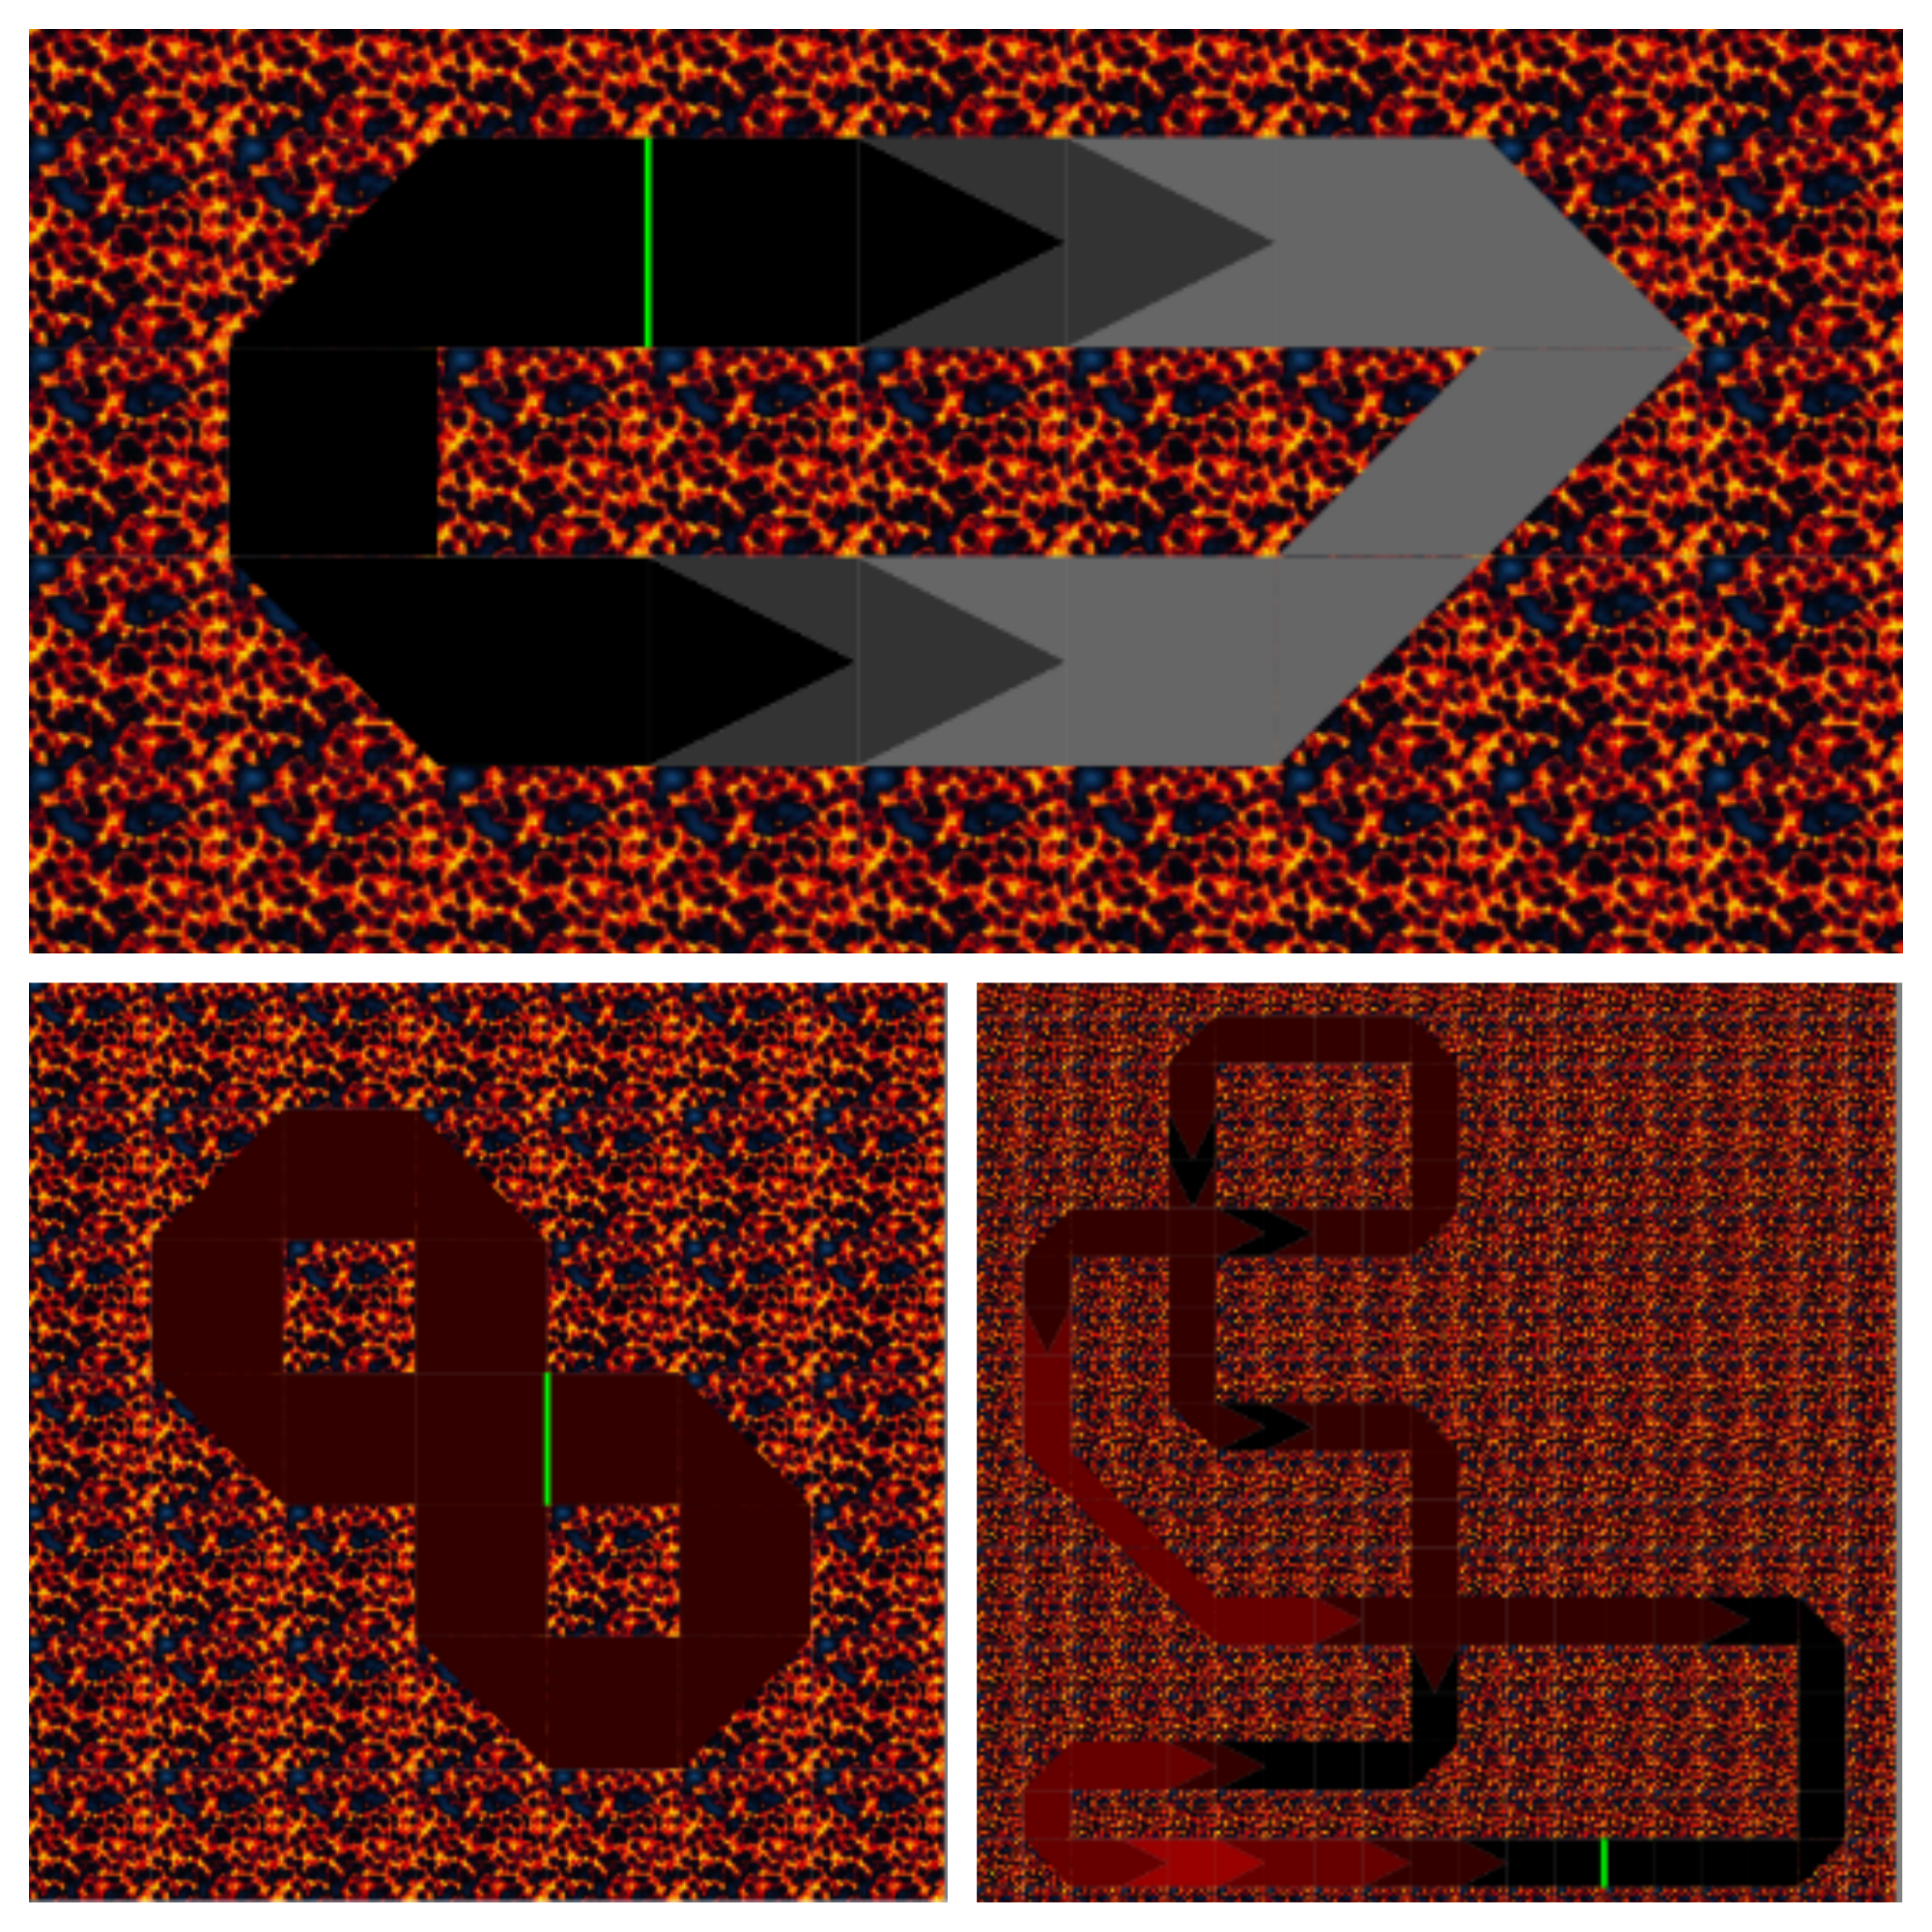
\includegraphics[scale=0.080]{Imagens/mapasV.png} \quad
  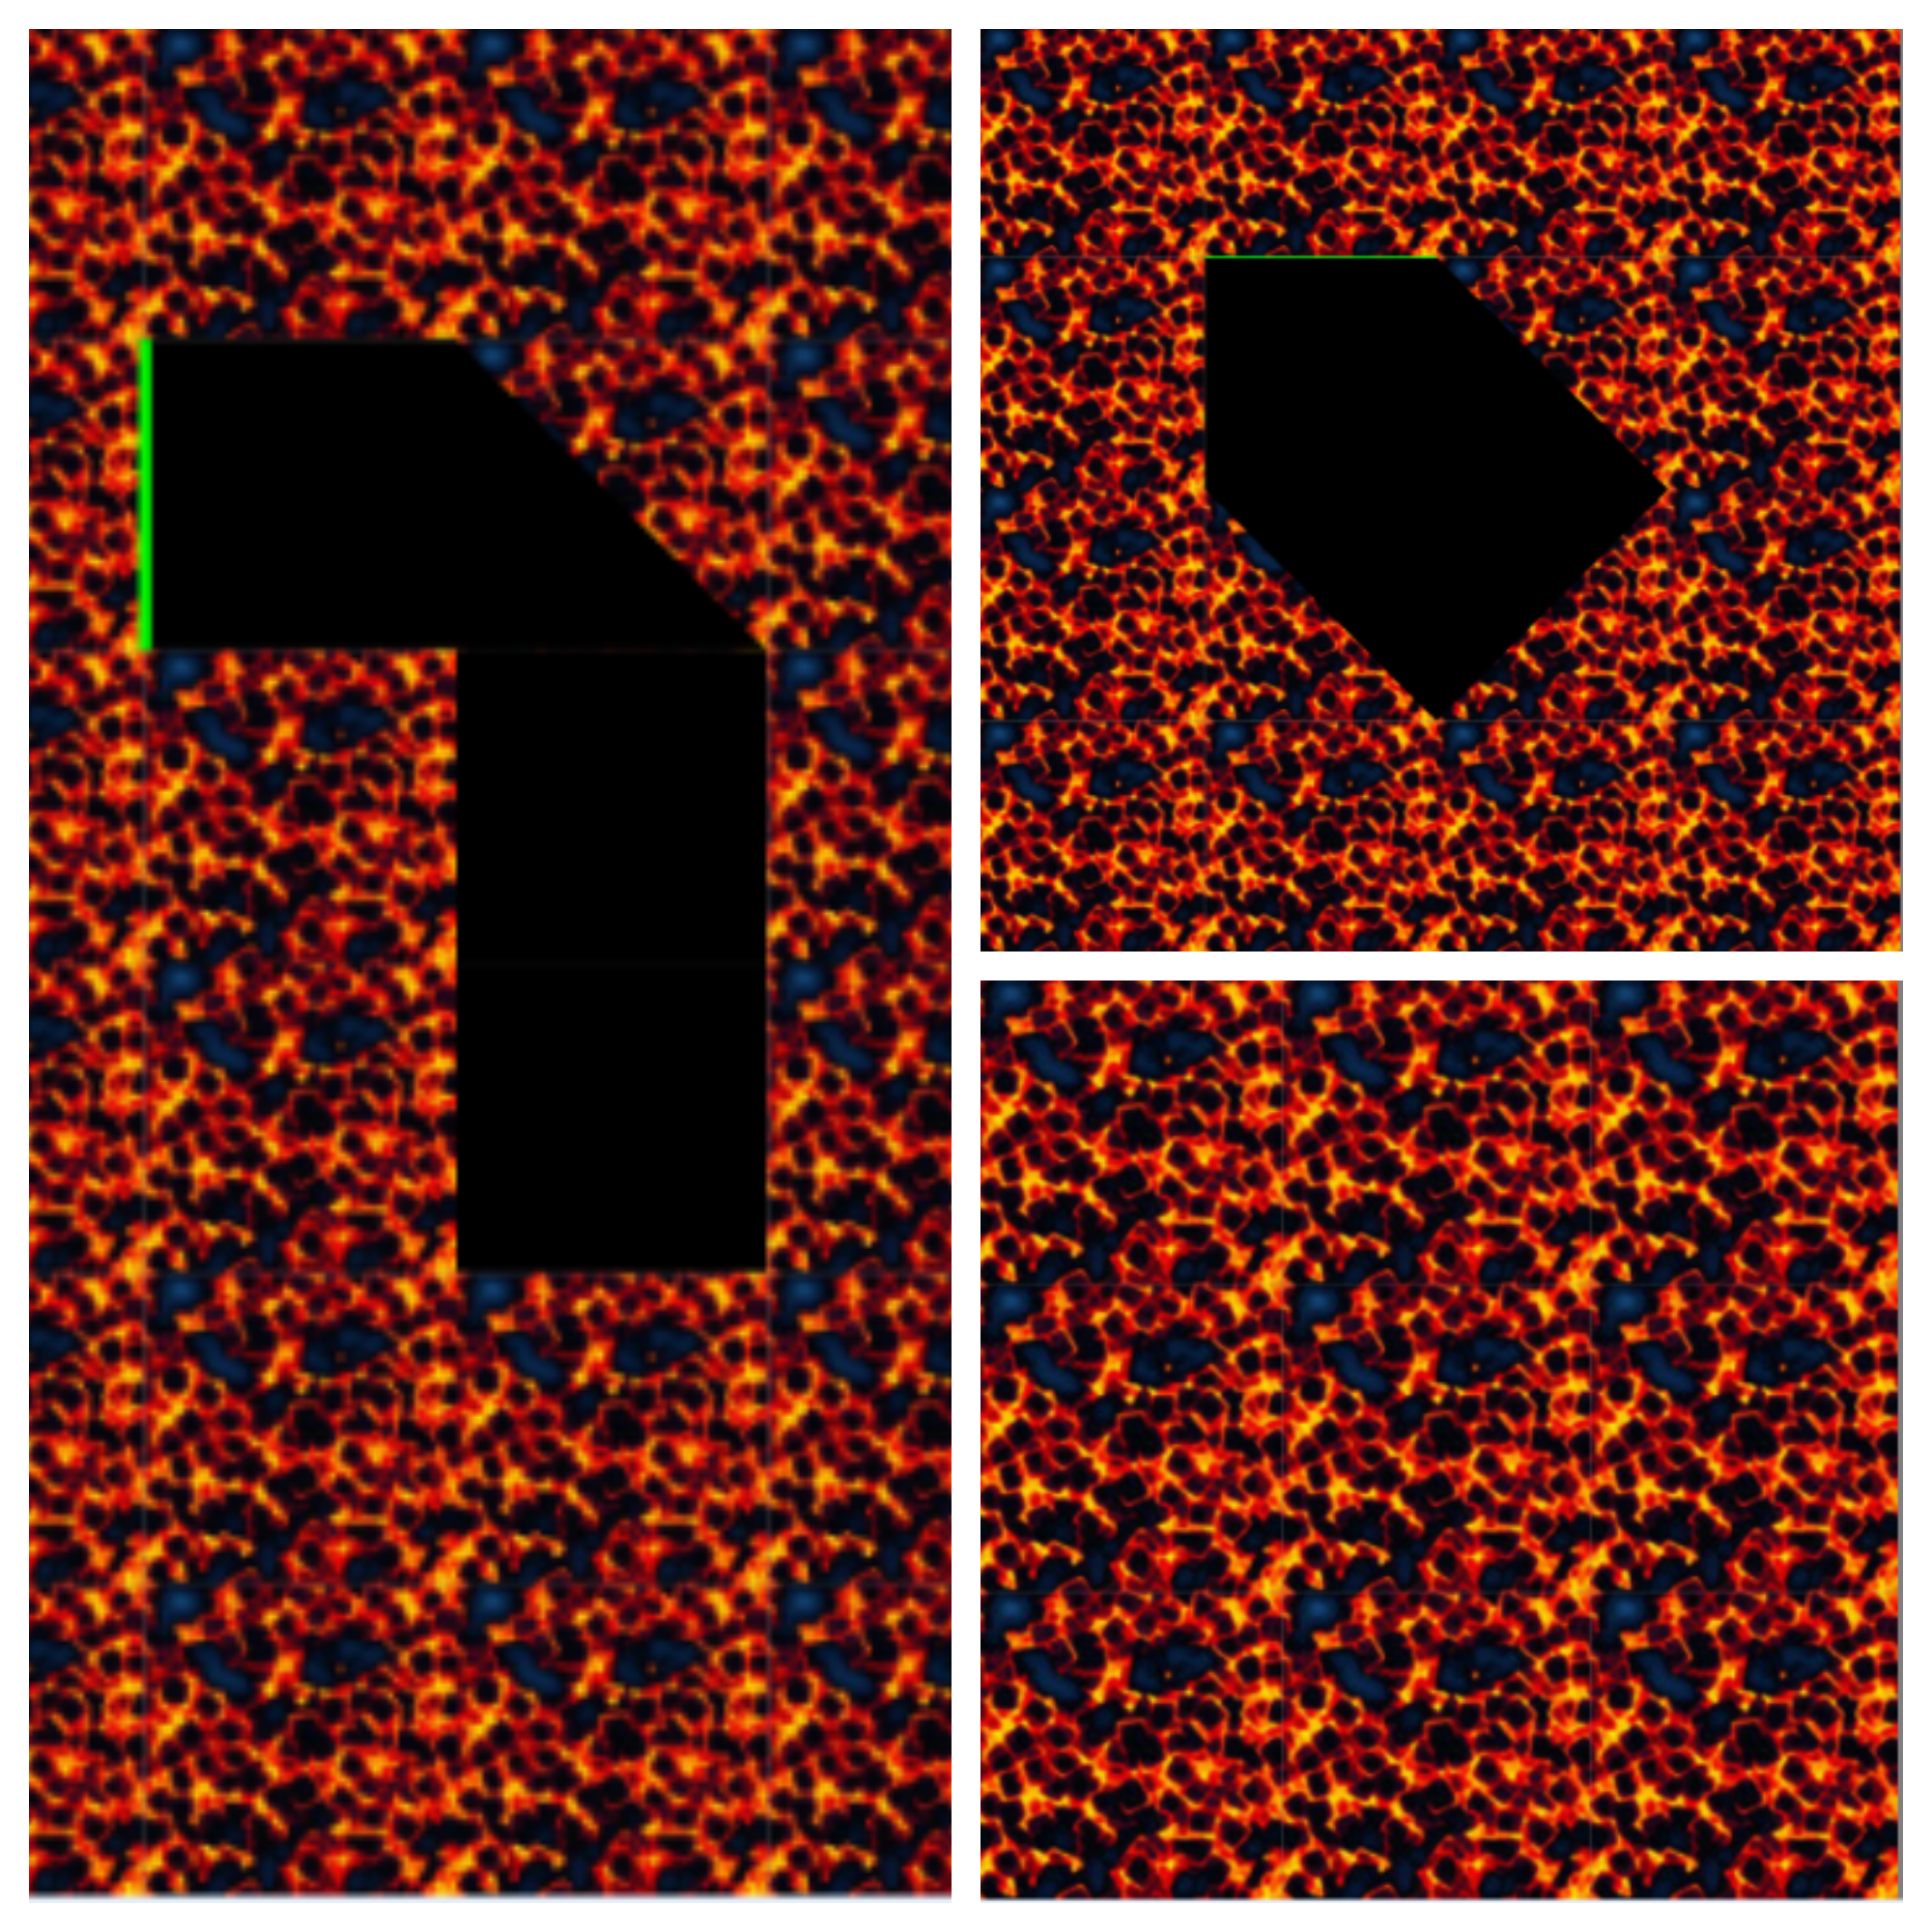
\includegraphics[scale=0.080]{Imagens/mapasInvalidos.png}
  \caption{Mapas Válidos (esquerda) e Inválidos (direita)} 
 
 \end{center}
 \end{figure}

 
 
\newpage
 
 \subsection{Tarefa 3}
 
 A derradeira etapa desta 1ºfase é a movimentação de um carro. Perante a ação de um jogador, o \emph{Carro} deve mover-se para a posição esperada. É necessário garantir que ocorre sua destruição quando estiver em contacto com a lava. Para além disso, deverá existir ricochete quando a diferença de alturas entre peças é superior a 1.
 
 O objetivo desta Tarefa é definir a função \textbf{movimenta}, que dado um \emph{Tabuleiro}, um \emph{Tempo} e um \emph{Carro},  devolve um \emph{Carro} correspondente. 

\begin{verbatim}
    
     movimenta :: Tabuleiro -> Tempo -> Carro -> Maybe Carro
     movimenta tab t c = isDestroyed tab (move t c)

\end{verbatim}

 \begin{figure}[!h]
    
    \centering
    \includegraphics[scale= 0.5]{Imagens/colisao.jpg}
    \caption{Movimentação do Carro}
 
 \end{figure}

\newpage

\section{Fase 2}
\label{sec:analisefasee}
 
\subsection{Tarefa 4}
 
 Para dar sucesão ao trabalho já realizado, é necesárrio implementar as consequências da movimentação do \emph{Carro}. Na Tarefa 4, pretende-se a criação da função \textbf{atualiza} que a partir de um jogo inicial, de um tempo, de uma ação e de um inteiro, identificativo do jogador em questão, devolve um novo jogo. 
 
 É importante que o aluno se aperceba da influência que as forças exercidas sobre o carro irão ter na alteração da sua velocidade. Pormenores como a direção e o sentido em que as forças são aplicadas no carro devem ser tidos em conta. Atenção também à presença da força do peso nas rampas.
 

\begin{figure} [!h]
    
    \centering
    \includegraphics[scale = 1.2]{Imagens/forcas.png}
    \caption{Forças aplicadas no Carro}

\end{figure}

O histórico (lista de listas de todas as posições em que os diferentes carros passaram) e a lista com os tempos de nitro de cada \emph{Carro} devem ser devidamente atualizadas. 

O cerne desta Tarefa é a definicão da função \textbf{atualiza}. Quando recebe um \emph{Tempo}, um \emph{Jogo}, um \emph{Int} e uma \emph{Acao}, a função devolve o \emph{Jogo} correspondente.

\begin{verbatim}
    
    atualiza :: Tempo -> Jogo -> Int -> Acao -> Jogo

\end{verbatim}

\newpage

 \subsection{Tarefa 5}

Na tarefa 5, a biblioteca \textit{Gloss} adiciona a cada grupo, uma panóplia de funções que possibilitam a edição gráfica do jogo. O executável deve ser apelativo e cada grupo tem a liberdade de implementar funcionalidades originais na sua animação. Esperam-se jogos autênticos. 

Nesta tarefa, a função \textbf{movimenta} e \textbf{atualiza} serão fundamentais para o bom funcionamento dos carros.

Pretende-se a definição da função \textbf{main} que devolve um \emph{IO ()}

\begin{verbatim}
  
   main :: IO ()

\end{verbatim}

\subsection{Tarefa 6}
Por fim, na Tarefa 6 é esperado que cada grupo implemente uma estratégia de  jogo para a movimentação dos bots.
    
    Para tal é necessário ter em conta que :
\begin{itemize}
    
    \item São permitidos atalhos , tendo em conta que estes não permitem a ultrapassagem de mais de 4 peças.
    \item A \emph{Velocidade} dos \textit{bots} deve ser inferior nas curvas relativamente a todas as outras peças.

\end{itemize}

Para que isso aconteça é nessecária a definição da função \textbf{bot}, que dado um \emph{Tempo}, um \emph{Jogo} e um \emph{Int}, devolve a \emph{Acao} resultante.

\begin{verbatim} 
    
    bot :: Tempo -> Jogo -> Int -> Acao

\end{verbatim}

%% Descrição da Solução Desenvolvida
\chapter{A Nossa Solução}
\label{sec:solucao}

\section {Fase 1}
\subsection {Tarefa 1}

\begin{table}[!h]
\begin{center}
\begin{tabular}{|l|c|r|}
    
    \hline
   \emph{Fases} & \emph{Descrição} & \emph{Função}\\
    \hline
    1º & Construção de um Tabuleiro de Lava & \textbf{buildLava} \\
    \hline
    2º & Posição das Peças & \textbf{passosToPosition} \\
    \hline
    3º & Escolhas das Peças & \textbf{passostoPecas} \\
    \hline
    4º & Alteração Local das Peças & \textbf{editTabuleiro} \\
    \hline
    5º & Construção do \emph{Tabuleiro} & \textbf{makeTabuleiro} \\
    \hline
    6º & Construção do \emph{Mapa} & \textbf{constroi} \\
    \hline
    
\end{tabular}
\end{center}
\caption{Fases da Resolução da Tarefa 1.}
\end{table}
 

 A chave para a realização de um \emph{Mapa} concordante com o \emph{Caminho} fornecido foi a criação de um algoritmo capaz de colocar peças na posição adequada do \emph{Tabuleiro}.
 
 Na maior parte dos casos, a \emph{Peca} que se repete mais vezes no \emph{Tabuleiro} é a \emph{Peca Lava 0}, pelo que foi intenção do grupo, criar uma função que a colocasse em todas as posições do \emph{Tabuleiro}.
 Para tal, necessitou-se de considerar as dimensão do \emph{Tabuleiro} correspondente ao \emph{Caminho} dado.
 
 Dessa forma, a primeira função a ser criada foi a função \textbf{buildLava}.
 
 \begin{verbatim}
     
     buildLava :: Caminho -> Tabuleiro
     buildLava c = let x = fst (dimensao c)
                       y = snd (dimensao c)  
              in  replicate y (replicate x (Peca Lava 0))

 \end{verbatim}

A inserção de \emph{CurvaDir} e \emph{CurvaEsq} no Caminho, faz com que se altere a \emph{Orientacao} que é tida em conta na construção das peças.

Devido a isso, houve a necessidade de elaborar uma função que colocasse as peças no local adequado, intitulada de \textbf{passosToPosition}. Devolve uma lista de \emph{Peca} a partir de um Caminho. Tem em conta \emph{Orientacao} inicial Este.

\begin{verbatim}
    
    passosToPosition:: Caminho -> [Posicao]
    passosToPosition [] = []
    passosToPosition c = positionEste (partida c) c

\end{verbatim}

Esta função está dependente de  outras 4 funções (\textbf{positionEste, positionOeste, positionNorte, positionSul}). Cada uma delas devolve a posição das peças segundo determinada \emph{Orientacao}. Recursivamente, devolvem as posições pretendidas.

Sob a influência do \emph{Caminho} está também a criação das peças que formam o Mapa. A \emph{Orientacao} volta a ser de novo fundamental, uma vez que o mesmo \emph{Passo} pode levar à execução de peças diferentes.

Para que a junção das peças seja a esperada comparativamente ao respectivo \emph{Caminho}, é necessário seguir um raciocínio similar ao da colocação das peças na \emph{Posicao} certa. Nas \textbf{pecasEste}, \textbf{pecasOeste}, \textbf{pecasNorte} e \textbf{pecasSul}) recursivamente irá ocorrer a formação de uma lista peças tendo em conta as diferentes orientações. A relação entre todas estas 4 funções irá ocorrer na função \textbf{passosToPecas}, que considera a \emph{Orientacao} inicial Este.

\begin{verbatim}
    
    passosToPecas :: Caminho -> [Peca]
    passosToPecas [] = []
    passosToPecas c = pecasEste 0 c
 
\end{verbatim}

Para relacionar todas as funções descritas anteriormente, necessitou-se de ter uma função que faz a substituição local de peças no \emph{Tabuleiro} de lava, apelidada de \textbf{editTabuleiro}. Para executar o primeiro passo recursivo, a função \textbf{insertPeca} faz a alteração da \emph{Peca} numa \emph{Posicao} especifica do \emph{Tabuleiro}.

Por fim, na função \textbf{makeTabuleiro} ocorre a construção do \emph{Tabuleiro}. Com isto chegou-se à função objetivo (\textbf{controi}), que dá um \emph{Mapa} em função de um \emph{Caminho}.

\begin{verbatim}
    
    makeTabuleiro :: Caminho -> Tabuleiro
    makeTabuleiro c = editTabuleiro (buildLava c)
    (passosToPecas c)(passosToPosition c)

\end{verbatim}    

\begin{verbatim}
    constroi :: Caminho -> Mapa
    constroi c = Mapa (partida c, Este) (makeTabuleiro c) 
\end{verbatim}
  

\newpage 
\subsection{Tarefa 2}
Para a resolução desta Tarefa, inicialmente houve a necessidade de certificar que o \emph{Mapa} em análise cumpria certos requisitos relacionados com a estrutura do seu\emph{Tabuleiro}.

Um \emph{Tabuleiro} é válido se o seu número de colunas for o mesmo em cada uma das linhas que o constitui. Para averiguar esta condição, o grupo criou a função \textbf{isValidTabuleiro}. Para além disso, esta função diz também que um \emph{Tabuleiro} vazio impossibilita a existência de um \emph{Mapa} válido.


A \emph{Peca} de partida não pode ser \emph{Peca Lava 0} e deve ter pelo menos uma \emph{Peca} adjacente que também não o seja.

Para completar as restrições relacionadas com a estrutura do \emph{Tabuleiro} a função \textbf{isBorderLava} certifica que as suas bordas são constituidas por \emph{Peca Lava 0}.

Todo o \emph{Mapa} é válido se for transitável, isto é, se for possiver ir desde a \emph{Peca} de partida até à \emph{Peca} final sem encontrar nenhuma \emph{Peca Lava 0}.

De maneira a descobrir se isto se verifica em qualquer \emph{Mapa}, o grupo criou a função \textbf{isValidPercorreMapa}. Esta função verifica primeiramente se a \emph{Peca} com a \emph{Posicao} imediatamente antes da partida é uma \emph{Peca} não lava. Se esta condição se verificar então  calcula o registo da passagem do carro com recurso à função \textbf{percorreMapa}, elimina as posições repetidas e substitui no mapa original todas as pecas que se encontram na lista por lava. Se o resultado for um tabuleiro só com lava e a última \emph{Posicao} da lista for a da partida então a função devolve o valor lógico de verdade.

Para obter o registo por onde o Carro passa, foi desenvolvida a função \textbf{percorreMapa} que simula um \emph{Carro} a percorrer o \emph{Mapa}. Esta função é chamada pela função \textbf{isValidPercorreMapa} e recebe o Mapa, um tuplo que contém a \emph{Posicao} imediatamente anterior à partida e a \emph{Orientacao} de partida. Ao longo dos passos recursivos este tuplo é utilizado para manter a  \emph{Posicao} e \emph{Orientacao} em que o \emph{Carro} se encontra e dois inteiros.

O primeiro inteiro tem o valor do dobro do número de peças não lava do \emph{Mapa}. Por cada passo de recursividade o valor diminui. Se este chegar a 0 é considerado como um caso de paragem e a função devolve no fim da Lista um Nothing. Tal impede que a função entre em ciclos infinitos sem conseguir voltar à partida com a \emph{Orientacao} inicial.

O segundo inteiro indica se o \emph{Carro} já passou uma vez pela partida ou não (Se ainda não passou o valor deste é 1, se já passou é 0). O valor que é passado pela função \textbf{isValidPercorreMapa} é sempre 1 pois, como o \emph{Carro} começa sempre nas coordenadas imediatamente antes da partida e a primeira passagem pela partida é ignorada.

Para que o \emph{Carro} avance para a próxima \emph{Peca} essa transição tem de ser válida. Para verificar se é posivel é utilizada a função \textbf{isValidNext}.

Se esta transição for válida, então a \emph{Posicao} do \emph{Carro} é adicionada à lista, e a função \textbf{percorreMapa} é chamada recursivamente, mas desta vez a \emph{Posicao} é a da próxima \emph{Peca} e a \emph{Orientacao}
é a que é dada pela função \textbf{dirChange}.

\newpage

\scriptsize

\begin{verbatim}
percorreMapa:: Mapa -> (Posicao, Orientacao) -> Int -> Int -> [Maybe Posicao]
percorreMapa m (p,o) 0 _ = [Nothing]
percorreMapa m@(Mapa (pi,oi) t) (p,o) v n 
| isValidNext m p o && coorNextPeca == pi && o == oi && n == 1 = Just p : percorreMapa m (coorNextPeca, dirChange m p o) 
(v - 1) (n - 1)
| isValidNext m p o && coorNextPeca == pi && o == oi && n == 0 = [Just p, Just coorNextPeca]
| isValidNext m p o = Just p : percorreMapa m (coorNextPeca, dirChange m p o) (v - 1) n
| otherwise = [Nothing]
            where
              coorNextPeca = nudge p o


\end{verbatim} 

\normalsize



A \textbf{isValidNext} devolve um Booleano que indica se o movimento é possivel atendendo à \emph{Posicao} e à \emph{Orientacao} que lhe é dada.

\begin{verbatim}

isValidNext::Mapa -> Posicao -> Orientacao -> Bool
isValidNext m p o | tipoPeca == Recta       = isValidReta  m p o
                  | tipoPeca == Curva Norte = isValidCurva m p o
                  | tipoPeca == Rampa Norte = isValidRampa m p o
                  | tipoPeca == Lava        = False
                    where
                      tipoPeca = tipoFinder (pecaFinder m (nudge p o))

\end{verbatim}

Dessa forma, temos tudo que é necessário para criar a função \textbf{valida}.

\begin{verbatim}

valida::Mapa -> Bool
valida m = isValidTabuleiro    m
        && isBorderLava        m
        && isValidPartidaPeca  m
        && isValidPercorreMapa m

\end{verbatim}
\newpage

\subsection{Tarefa 3}

Não pensando em possiveis colisões nem em destruições, o primeiro objetivo na Tarefa 3 foi fazer com que o carro se movesse. Em virtude disso mesmo, criou-se a função \textbf{move} que altera a \emph{Posicao} de um \emph{Carro} a partir do \emph{Tempo} dado. A soma das coordenadas da \emph{Posicao} do \emph{Carro} com o produto da coordenadas da \emph{Velocidade} pelo \emph{Tempo} foram a chave para obter uma \emph{Posicao} acertada. 

As destruições ocorrem quando o \emph{Carro} embate numa \emph{Peca Lava 0}. Dessa forma, o grupo apercebeu-se que em peças do \emph{Tipo} \emph{Curva Orientacao} esse fenómeno poderia ocorrer.

Por conseguinte, a função \textbf{isDestroyedCurva} certifica que o Carro é destruido assim que embate na diagonal de peças do \emph{Tipo} \emph{Curva Orientacao}. Foi necessário calcular a distância entre o \emph{Ponto} onde se situa o \emph{Carro} e a borda da \emph{Peca} onde este se encontra, através da função \textbf{coorInPeca}. Dependo da \emph{Orientacao} da curva, se o \emph{Ponto} onde se situa o \emph{Carro} estiver dentro da área englobada pela lava na \emph{Peca}, então a função \textbf{isDestroyedCurva} devolve \emph{Nothing}, acabando o \emph{Carro} por ser destruido.

Foi necessário relacionar a função \textbf{isDestroyedCurva} com uma função genérica ,\textbf{isDestroyed}, que nos diga quando é que o \emph{Carro} vai ser destruido. Para nos auxiliar tivemos a função \textbf{isCurva} que idetifica peças onde existem curvas. Nesses casos tivemos também em conta se a \emph{Altura} da \emph{Peca} era superior a 0. Se não o fosse, iria ocorrer ricochete.


\begin{verbatim}

isDestroyed:: Tabuleiro -> Carro -> Maybe Carro
isDestroyed t c | peca == Peca Lava 0 = Nothing
                | isCurva peca && altPeca >= 0 = isDestroyedCurva t c 
                | otherwise = Just c
            where
                peca = pecaTabFinder t c
                altPeca = alturaPeca peca

\end{verbatim}

Voltando ao raciocinio inicial, apenas faltava completar o algoritmo de forma a que as colisões ocorressem. Primeiramente criou-se a função \textbf{isRicochete} que identifica as situações onde ocorrem colisões, ou seja quando a diferença de alturas no \emph{Mapa} é superior a 0. Como a \emph{Direcao} do \emph{Carro} não se altera ao longo do jogo, faltava saber qual era a \emph{Posicao} para onde o Carro iria após o ricochete e qual a sua \emph{Velocidade}.

Sabendo qual o ponto de colisão, a descoberta do \emph{Ponto} para onde irá o \emph{Carro} faz-se multiplicando o \emph{Tempo} por cada uma das coordenadas desse ponto. 

Por falta de tempo, o grupo não conseguiu desenvolver uma função que calculasse qual a \emph{Velocidade} com que o \emph{Carro} chegaria ao respetivo \emph{Ponto} após a ocorrência de uma colisão. O grupo perpectivou que poderia calcular o vetor resultante da colisão, tendo que para isso considerar um vetor unitário no ponto onde ocorre o ricochete.

\begin{figure} [!h]
    
    \centering
    \includegraphics[scale = 1.2]{Imagens/velocidadeR.png}
    \caption{Cenário de Ricochete}

\end{figure}

\newpage

\section {Fase 2}

\subsection{Tarefa 4}

Para a atualização dos estado do jogo, à que ter em conta três novos \textit{datatypes}: o \emph{Jogo}, as \emph{Propriedades} e a \emph{Acao}.

\begin{verbatim}

data Jogo = Jogo 
{ mapa        :: Mapa         -- ^ o mapa do percurso
, pista       :: Propriedades -- ^ as propriedades do percurso
, carros      :: [Carro]      -- ^ o estado do carro de cada jogador
, nitros      :: [Tempo]      -- ^ a quantidade de nitro disponível para cada jogador
, historico   :: [[Posicao]]  -- ^ o histórico de posições de cada jogador
}

data Propriedades = Propriedades
{ k_atrito    :: Double -- ^ o atrito do piso
, k_pneus     :: Double -- ^ o atrito dos pneus 
, k_acel      :: Double -- ^ a intensidade da aceleração
, k_peso      :: Double -- ^ o efeito da gravidade nas rampas
, k_nitro     :: Double -- ^ a intensidade do nitro
, k_roda      :: Double -- ^ a sensibilidade do guiador
}
data Acao = Acao 
{ acelerar :: Bool      -- ^ Ativado quando o Carro acelera
, travar   :: Bool      -- ^ Ativado quando o Carro está a travar
, esquerda :: Bool      -- ^ Ativado quando o Carro curva à esquerda
, direita  :: Bool      -- ^ Ativado quando o Carro curva à direita
, nitro    :: Maybe Int -- ^ Ativado quando algum jogador dá Nitro
}

\end{verbatim}

As variações das ações dos jogadores alteram o \emph{Jogo}, nomeadamente os \emph{carros}, os \emph{nitros} e o \emph{historico}. Devido a isso, o grande objetivo da Tarefa 4 é que a atualização desses paramêtros ocorra de maneira acertada.

\newpage

\subsubsection{Atualização da Velocidade}

No que diz respeito às alterações que ocorrem nos \emph{carros}, o grupo devia criar funções capazes de atualizar a \emph{Velocidade} de cada um deles, bem como a sua \emph{Direcao}.

Considerem - se que os parâmetros do {datatype} \emph{Propriedades} podem representar forças aplicadas nos \emph{carros} ao longo do jogo. Cada um deles assume valores constantes.

O vetor velocidade do \emph{Carro} calcula-se a partir do somatório de todas as forças envolvidas, à excepção do k_roda e do k_nitro. O k_nitro apenas tem influência no valor do vetor velocidade se o nitro do jogador em questão for ativado. O k_peso também so é considerado em rampas.

O grupo decidiu trabalhar com coordenadas cartesianas, ao invés de utilizar coordenadas polares. Considerando as coordenadas polares como um tuplo, o elemento da esquerda representa a direção da força, ao passo que o elemento da direita é a sua norma. A função \textbf{vetAngToCoor} é responsável pela conversão.

\begin{verbatim}

vetAngToCoor:: VetorAng -> Vetor
vetAngToCoor (a,n) = (x, y)
            where
                x = n * cos (grauToRad a)
                y = - n * sin (grauToRad a)

\end{verbatim}



\maketitle\textbf{Forças Envolvidas}

\maketitle\underline{Aceleração}
\begin{table}[!h]
\begin{center}
\begin{tabular}{|l|c|r|}
    
    \hline
  \emph{Força} & \emph{Sentido} & \emph{Direção} \\
    \hline
  Aceleração & Igual ao do Carro & Igual à do Carro \\
    \hline

\end{tabular}
\end{center}
\caption{Aceleração.}
\end{table}

A direção e o sentido da aceleração são iguais às do \emph{Carro}. A norma é obtida multiplicando o \emph{Tempo} pela constante correspondente das \emph{Propriedades}, ou seja, o k_acel. Quando não existe aceleração, o valor devolvido pela função \textbf{acel} é (0,0).

\begin{verbatim}

acel::Bool -> Tempo -> Carro -> Propriedades -> Vetor  
acel b t car prop | b         = vetAngToCoor (direcao car, t * k_acel prop)
                  | otherwise = (0,0)

\end{verbatim}

\newpage

\maketitle\underline{Travagem}

\begin{table}[!h]
\begin{center}
\begin{tabular}{|l|c|r|}
    
    \hline
  \emph{Força} & \emph{Sentido} & \emph{Direção} \\
    \hline
  Travagem & Oposto ao do Carro & Igual à do Carro \\
    \hline

\end{tabular}
\end{center}
\caption{Travagem.}
\end{table}

Semelhante à Aceleração, com a particularidade de o seu sentido ser o oposto ao do \emph{Carro}. A norma obtem-te multiplicando o \emph{Tempo} pelo k_acel. Quando não existe aceleração, o valor devolvido pela função \textbf{trav} é (0,0).

\begin{verbatim}

trav::Bool -> Tempo -> Carro -> Propriedades -> Vetor
trav b t car prop | b         = vetAngToCoor ((direcao car) + 180, t * k_acel prop)
                  | otherwise = (0,0)

\end{verbatim}

\maketitle\underline{Atrito}

\begin{table}[!h]
\begin{center}
\begin{tabular}{|l|c|r|}
    
    \hline
  \emph{Força} & \emph{Sentido} & \emph{Direção} \\
    \hline
  Atrito & Oposto ao do Velocidade & Igual à da Velocidade \\
    \hline

\end{tabular}
\end{center}
\caption{Atrito.}
\end{table}

O ângulo da direção é o simétrico do ângulo da \emph{Velocidade}. A sua norma obtêm-se multiplicando o \emph{Tempo} pelo k_atrito e pela norma da velocidade.

\maketitle\underline{Força dos Pneus}

\begin{table}[!h]
\begin{center}
\begin{tabular}{|l|c|r|}
    
    \hline
  \emph{Força} & \emph{Sentido} & \emph{Direção} \\
    \hline
  Pneus & Oposto ao do Velocidade & Perpendicular à do Carro \\
    \hline

\end{tabular}
\end{center}
\caption{Força dos Pneus.}
\end{table} 

A direção é perpendicular à do \emph{Carro}, logo o ângulo da direção do Pneu pode ser superior ou inferior relativamente ao ângulo da direção do \emph{Carro}.
Considere-se as duas situações :

\begin{itemize}
   
   \item Quando o ângulo da direção do vetor \emph{Velocidade} é superior ou igual ao ângulo da direção do \emph{Carro}, subtrai-se 90 graus a este último para obter o ângulo da direção da força do Pneu.
   \item Caso contrário, soma-se 90 graus ao ângulo da direção do \emph{Carro}.

\end{itemize}

A sua norma obtêm-se multiplicando o \emph{Tempo} pelo k_pneus.

\newpage

\maketitle\underline{Gravidade}

\begin{table}[!h]
\begin{center}
\begin{tabular}{|l|c|r|}
    
    \hline
  \emph{Força} & \emph{Sentido} & \emph{Direção} \\
    \hline
  Gravidade &  Igual ao do declive da Rampa & Igual ao do declive da Rampa \\
    \hline

\end{tabular}
\end{center}
\caption{Gravidade.}
\end{table}

Para descobrir o ângulo corresponde ao declive da Rampa em questão, o grupo utilizou a função \textbf{orToAng}. Consoante a \emph{Orientacao} da Rampa, a função devolve um \emph{Double} correspondente ao valor do ângulo.

\begin{verbatim}
orToAng:: Orientacao -> Double
orToAng Norte = 90 
orToAng Sul   = 270
orToAng Este  = 0
orToAng Oeste = 180
\end{verbatim} 

O valor da norma da gravidade correponde à multiplicacão do \emph{Tempo} pelo k_peso.

Conhecidas todas as particularidades das forças envolvidas para a atualização do vetor velocidade, o grupo decidiu organizar as coordenadas cartesianas de cada uma delas numa lista. Na função \textbf{vetorRes} é calculado o somatório de todas as coordenadas presentes dentro da lista anteriormente referida. Tal não seria possivel sem a função \textbf{sumVet}, que soma os vetores existentes dentro de uma lista.

\begin{verbatim}

vetoresRes::Tempo -> Jogo -> Int -> Acao -> [Vetor]
vetoresRes t j i a = [(vx,vy),
                      acel (acelerar a) t car prop,
                      trav (travar a)   t car prop,
                      peso isPeso t car prop anVetPeso,
                      pneu t car prop,
                      atrito]
             where
                m         = mapa j
                prop      = pista j
                car       = (carros j) !! i
                (vx,vy)   = velocidade car
                (va, vn)  = vetCoorToAng (velocidade car)
                pecaLocal = pecaFinder m (coorPeca car)
                isPeso    = tipoFinder pecaLocal == Rampa Norte (*)
                atrito    = vetAngToCoor (va - 180, t * vn * (k_atrito prop))
                anVetPeso = orToAng (orFinder pecaLocal Norte) - 180

(*) Rampa Norte é o resultado que a função tipoFinder devolve para peças do tipo Rampa.


vetorRes:: Tempo -> Jogo -> Int -> Acao -> Vetor
vetorRes t j i a = sumVet (vetoresRes t j i a)

\end{verbatim}

\subsection{Atualizar a quantidade de Nitro}

A direção do vetor do nitro é a mesma que a direção do vetor do \emph{Carro}. A sua norma é dada pela multiplicação do \emph{Tempo} pelo k_nitro.

\begin{verbatim}

nit::Bool -> Tempo -> Carro -> Propriedades -> Vetor
nit b t car prop | b         = (vetAngToCoor (direcao car, t * k_nitro prop))
                 | otherwise = (0,0)

\end{verbatim}

A ativação do nitro leva a que o vetor velocidade seja alterado. A este será adicionado o vetor do nitro. A alteração da velocidade em cada um dos \emph{carros} é feita de forma análoga à substituição de peças no Tabuleiro, na Tarefa 1. Primeiramente retira-se a parte da lista de \emph{carros} que não vai ser alterada até à posição da lista onde irá ocorrer a substuição. De seguida, ocorre a mudança do vetor velocidade no \emph{Carro} em que o nitro é ativado. Por fim devolve-se a lista de carros restante, que não irá sofrer nenhuma alteração. A função \textbf{atList} é a responsável pela realização deste processo na função \textbf{applyNit} que funciona quando o nitro é ativado.

\scriptsize

\begin{verbatim}

applyNit::Tempo -> [Carro] -> [Tempo] -> Propriedades -> Int -> Acao -> [Carro]
applyNit t cars tNit prop i a | nitID == Nothing = cars
                              | otherwise = atList cars (car {velocidade = (vx + nx, vy + ny)}) (fromJust nitID)
            where
                nitID    = nitro a
                car      = cars !! (fromJust nitID)
                (vx, vy) = velocidade car
                (nx, ny) = nit ((tNit !! i) > 0) t car prop

\end{verbatim}

\normalsize

A função \textbf{tNitDiscount} ficou encarregue de descontar o tempo de nitro de cada jogador. Calcula a diferença entre o tempo dado e o valor de tempo de nitro final do jogador em questão. Com a ajuda de uma função auxiliar, sempre que a diferença for inferior a 0, a função \textbf{tNitDiscount} impossibilitava a ocorrência de mais nitro.


\scriptsize

\begin{verbatim}

tNitDiscount:: Tempo -> Jogo -> Int -> Acao -> [Tempo]
tNitDiscount t j i a | isNit     = atList listTNits tNitFinal i
                     | otherwise = listTNits         
            where
                isNit     = (nitro a) /= Nothing
                tNitCar   = (listTNits) !! i
                listTNits = nitros j
                tNitFinal = aux (tNitCar - t)
                            where
                                aux:: Double -> Double
                                aux t | t < 0     = 0
                                      | otherwise = t

\end{verbatim}

\newpage

\normalsize

\subsubsection{Atualizar Direção}

Através da mudança do valor booleano do parâmetro esquerda ou direita da \emph{Acao}, altera-se também a direção do \emph{Carro}. Dessa forma, ao ângulo da direção irá ser somado um novo valor, que se obtêm multiplicando o \emph{Tempo} pelo k_roda.

\scriptsize

\begin{verbatim}

dirCarChange::Tempo -> Jogo -> Int -> Acao -> Double
dirCarChange t j i a | esq && dir = dirCar
                     | esq        = dirCar + deltaD
                     | dir        = dirCar - deltaD
                     | otherwise  = dirCar
            where
                dirCar = direcao ((carros j) !! i)
                esq    = esquerda a
                dir    = direita a
                prop   = pista j 
                deltaD = t * k_roda prop

\end{verbatim}

\normalsize

Tendo a funções necessárias para a atualização da \emph{Direcao} e da \emph{Velocidade}, tem-se tudo que é preciso para atualizar o \emph{Carro}.
A velocidade pode-se alterar em função da ativação do nitro.
A função \textbf{atCarros} devolve o \emph{Carro} atualizado, mesmo que este esteja sobre a influência do nitro.

\scriptsize

\begin{verbatim}

atCarros::Tempo -> Jogo -> Int -> Acao -> Jogo
atCarros t j i a = j {carros = applyNit t carNotNit tNit prop i a}
            where
                m         = mapa j
                prop      = pista j
                car       = (carros j) !! i
                v         = velocidade car
                dCha      = dirCarChange t j i a
                vRes      = vetorRes  t j i a
                tNit      = nitros j
                carNotNit = atList (carros j) (car {direcao = dCha, velocidade = vRes}) i

\end{verbatim}

\newpage

\normalsize

\subsubsection{Atualizar o Histórico}

O histórico é uma lista das posições por onde o que \emph{Carro} já passou e é atualizado em função da alteração da \emph{Acao}. A nova \emph{Posicao} é sempre colocada na cabeça da lista.

\begin{verbatim}

atHist:: Carro -> [Posicao] -> [Posicao]
atHist c log | head (log) == coorCarro = log
             | otherwise               = [coorCarro] ++ log
             where
                 coorCarro = coorPeca c

\end{verbatim}

Todas as estas funções irão se relacionar na função \textbf{atualiza}.

\begin{verbatim}

atualiza t e j a = atCarros t atHistNit j a
                where
                    carroHistNew = atHist carroTarget carroHistOld
                    carroTarget  = (carros e) !! j
                    carroHistOld = jogoHistOld !! j
                    atHistNit    = e {nitros = tNitNew, historico = jogoHistNew}
                    tNitNew      = tNitDiscount t e j a
                    jogoHistNew  = atList jogoHistOld carroHistNew j
                    jogoHistOld  = historico e

\end{verbatim}

\normalsize

\newpage

\subsection{Tarefa 5}

Após a análise da documentação referente à biblioteca \textit{Gloss}, verificámos que para a realização desta Tarefa seria necessário utilizar a função \textbf{play}, pré-definida no \textit {package} "Graphics.Gloss.Interface.Pure.Game".

\scriptsize 
 
 \begin{verbatim}

play :: Display  

-> Color  
Cor do Fundo.

-> Int  
Frame Rate.

-> world  
O "mundo" inicial.

-> (world -> Picture) 
Uma função para converter o world para uma Picture.

-> (Event -> world -> world)  
Uma função que reage a eventos.

-> (Float -> world -> world)  
Uma função que devolve um determinado world após a passagem do Tempo que lhe é dado.

-> IO ()
O resultado final.

\end{verbatim}

\normalsize

Dessa forma, o grupo criou a função \textbf{joga}, onde se relacionam todas as funções que permitem a criação do executável do jogo. Esta função está dependente da função \textbf{play}, acima descrita.

Para a utilização da função \textbf{play} tivemos de criar um \textit{datatype} que funcionasse como \emph{world}. Apelidámo-lo de \emph{Estado} e está definido sobre a forma de \textit{record}.

\scriptsize

\begin{verbatim}

data Estado = Estado
              { jogo     :: Jogo          -- ^ Principais parâmetros do jogo
              , actions  :: Actions       -- ^ Ações dos jogadores
              , images   :: Images        -- ^ Imagens do Jogo
              , nPlayer  :: Int           -- ^ Indica o número de jogadores não bot presentes
              , camera   :: Camera        -- ^ Tipo de câmera onde decorre a corrida
              , winSize  :: (Int, Int)    -- ^ Contém o tamanho da janela em que o jogo está a correr
              , pausa    :: Bool          -- ^ Indica se está em pausa ou não
              , inCountDown :: Bool       -- ^ Indica se está em contagem decrescente para começar ou não
              , tToStart    :: Float      -- ^ Indica quanto tempo falta para começar
              , tFromStart  :: Float      -- ^ Indica quanto tempo é que passou desde que o jogo começou
              , inMenu      :: Bool       -- ^ Indica se está dentro de um dos Menus do jogo
              , whereMenu   :: MenuPos    -- ^ Indica em qual dos Menus se encontra 
              , pMapa       :: Caminho    -- ^ O caminho para a formação de mapas pelo jogador
              , nVoltas     :: Int        -- ^ Indica o número de VOltas a dar pelo utilizador
              , idPath      :: [Posicao]  -- ^ Indica o caminho ideal de uma volta à pista (utilizado para contar voltas) 
              }

\end{verbatim}

\normalsize
Nas paginas seguintes falaremos das etapas da elaboração desta fase do projeto, sendo especificado a utilidade dos diferentes parâmetros do \emph{Estado}.

\newpage

O jogo subdivide-se em dois diferentes momentos: o momento da corrida, que foi criado através da funcão \textbf{desenhaJogo}, e a parte em que o utilizador do executável se encontra num dos menus dos jogo. A função que ficou encarregue por desenhar o menus foi a \textbf{desenhaMenus}

Estas duas funções irão se relacionar na função \textbf{desenhaEstado} que irá construir tudo aquilo que aparece no ecrã.

\begin{verbatim}

desenhaEstado :: Estado -> Picture
desenhaEstado e | inMenu e  = desenhaMenu e
                | otherwise = desenhaJogo e

\end{verbatim}

As diferentes fases que levaram o grupo a chegar à função pretendida estão sintetizadas no quadro seguinte.


\begin{table}[!h]
\begin{center}
\begin{tabular}{|c|c|}
    \hline
  \emph{Etapa} & \emph{Objetivo} \\
    \hline
  1º & Construção de mapas \\
    \hline
  2º & Colocação dos carros nos mapas \\
    \hline  
  3ª & Extras no Modo Corrida \\
    \hline
  4ª & Desenho dos Menus \\
    \hline
  5º & Extras nos Menus \\
    \hline

\end{tabular}
\end{center}
\caption{Fases da Elaboração da \textbf{desenhaEstado}.}
\end{table}


\subsubsection{Elaboração da \emph{desenhaJogo}}

\maketitle\underline{Construção dos Mapas}

O primeiro passo na resolução desta tarefa foi criar uma função que permitisse gerar qualquer mapa no ecrã a partir de um \emph{Tabuleiro}.
Para tal o grupo desenhou as diferentes peças que fazem parte do \emph{Tabuleiro}.

Cada peça é um quadrado. Em virtude do \emph{Tabuleiro} dado, o lado deste quadrado irá se alterar, pelo que não existia um valor fixo que o grupo lhe poderia atribuir. 

A função \textbf{sizePeca} dá o valor do lado de cada peça. Dada uma janela do ecrã, e um \emph{Tabuleiro} a função descobre qual o valor máximo que o lado pode tomar, atendendo ao números de peças que irão existir horizontalmente (comprimento da cabeça do \emph{Tabuleiro}) e verticalmente (comprimento do \emph{Tabuleiro}) 

Depois disso, seleciona o menor dos dois valores encontrados, garantindo assim que todas as peças cabem no ecrã.

\begin{verbatim}

sizePeca:: Tabuleiro -> (Int,Int) -> Int
sizePeca a@(l:t) (x,y)= minimum [maxX, maxY]
            where
              maxX = floor ((fromIntegral y)/ fromIntegral (length a))  
              maxY = floor ((fromIntegral x)/ fromIntegral (length l))

\end{verbatim}

\newpage

Para o desenho das peças à que considerar 4 grupos de peças : retas, curvas, rampas e lava.

As retas fazem-se através da função \textbf{polygon}, que desenha um poligono em virtude das coordenadas dadas. Importante referir, que nas coordenadas dadas, a cabeça e o último elemento devem ser iguais.

\begin{verbatim}

reta :: Int -> Picture
reta l = Polygon [(-r,-r),(r,-r),(r,r),(-r,r),(-r,-r)]
            where
              r = fromIntegral l / 2

\end{verbatim}

As curvas são feitas segundo o mesmo mecanismo. As coordenadas que constituem a lista dada à função \textbf{polygnon} é que é são diferentes.

\scriptsize

\begin{verbatim}
               
curvaNorte :: Int -> Picture
curvaNorte l = Polygon [(-r,-r),(r,-r),(r,r),(-r,-r)]
            where
              r = fromIntegral l / 2
\end{verbatim}

\normalsize

As rampas necessitam da função \textbf{pictures}, que forma uma imagem através da junção de várias figuras. Na lista de figuras dadas, foi necesário criar um identificativo das rampas, que neste caso foi a imagem que forma 2 triângulos paralelos. Houve a nessecidade de aplicar a função \textbf{translate} que move um figura segundo as coordenadas dadas.

\scriptsize

\begin{verbatim}

rampaNorte :: Int -> Picture
rampaNorte l = Pictures[reta l, arrow1, arrow2]
            where
              r = fromIntegral l/2
              arrow1 = color colorarrow (Polygon [(0,0),(r, -r/2), (r,-r), (0,-r/2), (-r,-r),(-r,-r/2), (0,0)])
              arrow2 = Translate 0 r arrow1
              colorarrow = greyN 0.5

\end{verbatim}

\normalsize

A lava é uma figura em branco. Utiliza-se a função \textbf{blank}, pré-definida no \textit{Gloss}.

\begin{verbatim}

lava :: Picture
lava = blank

\end{verbatim}

O grupo optou por fazer a construção do mapa no ecrã de forma recursiva.
Primeiro era necessário fazer a construção de uma linha de peças, para ocorrer a repetição deste processo nas restantes linhas.

A primeira linha é feita com a função \textbf{drawline}. Esta necessita da função \textbf{placePeca} para colocar as peças no local certo.

\begin{verbatim}

drawLine :: Int ->[Peca] -> Picture
drawLine s l = Pictures (placePeca s translationX (map (desenhaPeca s) l))
            where
              translationX = -(fromIntegral(length l)/2)* (fromIntegral s)

\end{verbatim}

\newpage

Para construir o restante mapa, o raciocinio é análogo à construção de uma linha de peças.
Neste caso teremos a função \textbf{drawlines}, que com o auxilio da \textbf{placelines}, coloca as linhas de peças no sitio certo do ecrã.

\begin{verbatim}

drawLines :: Int -> Tabuleiro -> Picture
drawLines s t = Pictures (placeLines s translationY (map (drawLine s) t))
            where
              translationY = (fromIntegral(length t)/2)* (fromIntegral s)

\end{verbatim}

Construida em último lugar mas não menos importante, vem a colocação da linha de partida. A função \textbf{startLine} recebe o lado de cada peça, conseguindo desta forma fazer o desenho da partida.

Devido à sua extensão não a colocaremos neste relatório. De destacar que utilizámos uma função do \textit{Gloss} ainda não mencionada, a função \textbf{color}. Ela aplica uma cor uma \emph{picture}. Neste caso, foi necessária para que poligonos adjacentes ficassem com cores diferentes, de maneira a formar uma imagem semelhante a uma linha de partida.

\normalsize

Depois de tudo isto, basta fazer a função final que irá, efetivamente, desenhar o mapa no ecrã. 

\scriptsize

\begin{verbatim}

drawMapa:: Estado -> Picture
drawMapa e = Pictures [drawLines pSize tab, start]
            where
              (Mapa (p,o) tab) = (mapa (jogo e))
              (px,py) = p
              (sx,sy) = (fromIntegral px + 0.5, fromIntegral py + 0.5)
              pSize = sizePeca tab (winSize e)
              (x,y) = cornerToCenter pSize tab (sx, sy) 
              start = Translate (realToFrac x) (realToFrac y) (startLine pSize)

\end{verbatim}

\normalsize

\newpage

\maketitle\underline{Colocação dos carros nos mapas} 

As coordenadas da \emph{Posicao} dos carros são dadas a partir de um referencial que tem a origem no canto superior esquerdo do ecrã.

O \textit{Gloss} tem em conta que todas as coordenadas dados tem como ponto (0,0) o centro do ecrã.

Dessa forma, o grupo criou a função \textbf{cornerToCenter}.

Esta função funciona com base em vetores.

Primeiramente, multiplica-se as coordenadas dadas pelo tamanho da \emph{Peca} em pixeis.

Em seguida, usando como referencial o canto superior esquerdo, calcula-se as coordenadas do centro do ecrã. Este será a origem do referencial para o qual queremos converter.

Por fim, calcula-se as coordenadas do vetor que vai da origem do referencial no centro do mapa, para as coordenadas do carro em pixeis.

No entanto, ocorre inversão do eixo das ordenadas. Para isso ser contabilizado, o valor devolvido do y é o simétrico do vetor calculado anteriormente.

\begin{verbatim}

cornerToCenter::Int -> Tabuleiro -> Ponto -> Ponto
cornerToCenter pSize tab (x,y) =( cx + p * x,cy - y * p) 
            where
              cy = ((fromIntegral(length tab)/2) + 0.5 )* p
              cx = (-(fromIntegral(length (head tab))/2) - 0.5) * p
              p = fromIntegral pSize

\end{verbatim}

\normalsize

A função \textbf{drawCar} através da conjugação de um \textbf{translate}, em que os valores dos \textit{floats} são as coordenadas onde o \emph{Carro} se encontra, com um \textbf{rotate}, que permite que o \emph{Carro} rode até ao simétrico da sua \emph{Direcao}, desenha um carro no mapa do ecrã.

\scriptsize

\begin{verbatim}

drawCar:: Estado -> [Picture] -> Int -> Picture
drawCar e picCars i = Translate (realToFrac x) (realToFrac y) (Rotate (realToFrac a) pic)
            where
                tab     = mapToTab (mapa (jogo e))
                listCar = carros(jogo e)
                (x,y)   = cornerToCenter pSize tab (posicao (listCar !! i))
                a       = -1 * direcao (listCar !! i)
                pic     = scale fs fs (picCars !! i)
                pSize   = sizePeca (mapToTab (mapa (jogo e))) (winSize e)
                fs      = fromIntegral pSize * 0.50 / 2400

\end{verbatim}

\normalsize

Na função \textbf{drawCars} irá ser aplicada a função \textbf{drawCar} a cada um dos carros.

\newpage

\maketitle\underline{Extras no Modo de Corrida}

É no modo de corrida onde se encontram a maior parte dos extras do jogo.

Começamos por explicar aquele que nos obrigou a criar um \emph{datatype} novo, designado de \emph{Camera}. Ele é o tipo que define o parâmetro \emph{camera} do \emph{Estado}. 

No modo corrida, o jogador tem a possibilidade de alterar a câmera com que visualiza o jogo. Existem 3 opções: \emph{full}, câmera pré-definida para o inicio da corrida, \emph{close}, que efetua zoom sobre o jogador em questão e \emph{birdEye}, na qual o jogador vê o jogo através de uma perspectiva superior à dos carros, ou por outras palavras, "vê os carros vistos de cima".

Para fazer a câmera em modo \textit{close} basta aplicar um \textbf{translate} à imagem que desenha os carros e o mapas. Os dois \textit{floats} que o \textit{translate} irá receber serão o simétrico da coordenadas onde se encontra o carro.

Em modo \emph{birdEye} aplica-se um \textbf{rotate} à imagem formada no modo \textit{close}. Essa rotação irá ocorrer segundo o ângulo da direção inicial do carro, menos 90 graus.

É possivel também colocar o jogo em Pausa. Basta que o parâmetro \emph{pausa} do \emph{Estado} seja verdadeiro. Quando isso acontece irá ser ativado o parâmetro pauseMenu (que faz parte do \textit{datatype} Images) alterando as \emph{images} do \emph{Estado}. O \textit{datatype} \emph{Images} foi criado para armazenar todas as imagens que serão necessárias no jogo.

Cada jogador terá um identificativo no canto superior direito do ecrã, com o respectivo nitro. Estes identificadores aparecerão ordenados consoante a posição do carro do jogador na corrida. O nitro será renovado sempre que o jogador acabar de dar uma volta à pista.

Mais à frente será abordado de uma forma mais especifica, mas em virtude deste tópico, refere-se já que existirão 3 niveis de dificuldade.
No nivel mais fácil, o jogo terminará após 3 voltas à pista. No nivel intermédio, acabará com 2 voltas ao circuito e no nivel mais avançada apenas será necessário completar uma volta.

\newpage

No ecrã estará também o número de voltas percorridas pelo jogadores. Esse número corresponderá ao nº de voltas do jogador que se posiciona em primeiro lugar. A função responsável pelo desenho é a \textbf{drawLapCount}, que em virtude do \emph{nVoltas} que recebe do \emph{Estado}, desenha no ecrã o número correspondente. Na última volta à pista, em vez de aparecer o número, aparece a expressão \textit{"final lap"}.

Para que a função \textbf{drawLapCount} saiba o que deve reproduzir no ecrã, auxiliou-a a função \textbf{lapCountList}. Esta função devolve o número de voltas dadas por cada jogador. Para saber o que desenhar, a função \textbf{drawLapCount} retira o maior número da lista de inteiros devolvida pela \textbf{lapCountList} e adiciona-lhe 1, uma vez que o inteiro a que corresponde o número de voltas dadas por cada jogador, só se altera quando o \emph{Carro} termina a volta em que se encontra. No visor deve aparecer o número dessa volta.

Por fim, o jogador poderá também ver no ecrã um cronómetro com o tempo desde o inicio da partida. Mais uma vez, utilizá-mos para nos auxiliar uma função pré-definida no \textit{Gloss}, a função \textbf{text}, que dada uma \emph{string} a coloca no ecrã. A \emph{string} que irá receber corresponderá ao valor do parâmetro tFromStart definido no \emph{Estado}.

Desta forma, todas as funções que permitem o funcionamento da função \emph{desenhaJogo} já foram explicadas. Em virtude do tamanho da sua definição não a iremos apresentar. Contudo, fica o sumário das situações em que esta função é ativada.

\begin{itemize}

    \item Desenhar o jogo em \textit{CountDown};
    \item Desenhar o jogo em em pausa;
    \item Desenhar o jogo nas diferentes câmeras.

\end{itemize}  

\newpage

\subsubsection{Elaboração da \emph{desenhaMenus}}

Para a construção dos menus será fundamental o parâmetro \emph{whereMenu} presente no \emph{Estado}. Na função \textbf{desenhaMenu} estarão programadas as imagens respectivas ao menu que o jogador selecionar.

O grupo utilizou a função \textbf{scale} para escalar as imagens dos menus. Foram utilizados dois pares de valores diferentes para os escalonamento das \emph{pictures}. 

À excepção do desenho do \textit{help} no menu inicial, os valores de escalanomento foram o valor minimo entre ,a divisão do coordenadas da janela dada a partir do \emph{winSize}, e 2048.

\begin{figure}[h!]

  \centering
  \includegraphics[scale= 0.4]{Imagens/Inicio.png}
  \caption{Menu Inicial}

\end{figure}

Em relação ao caso que é excepção o que foi dito em cima, os valores utilizados foram na mesma o minimo da divisão de cada uma das coordenadas da \emph{winSize}, mas desta vez por valores mais elevados, em virtude do tamanho da palavra \textit{help}.

Quando a corrida termina, um novo menu aparece no ecrã. A função responsável pela sua formação é a \textbf{desenhaMenuEndGame}. Os jogadores irão aparecer no ecrã conforme a sua posição no final da corrida. Para isso a auxiliar esta função vem a \textbf{listIDs} que dá uma lista ordenada dos carros consoante a sua posição no jogo. 

Em baixo dessa lista aparecerá o simbolo do \textit{enter}, obtido através do parâmetro \emph{extraCreate} definido no \textit{datatype} \emph{Images}. 

\newpage

\subsubsection{Elaboração da \textbf{reageTempo}}

\begin{table}[!h]
\begin{center}
\begin{tabular}{|c|c|}
    \hline
  \emph{Etapa} & \emph{Objetivo} \\
    \hline
  1º & \emph{Ponto} onde se encontra \emph{Carro} após as Destruições \\
    \hline
  2º & Implementação da função \emph{movimenta} \\
    \hline  
  3ª & Implementação da função \emph{atualiza}\\
    \hline
  5º & Tempos antes e após a corrida\\
    \hline

\end{tabular}
\end{center}
\caption{Fases de Elaboração da \emph{reageTempo}}
\end{table}


Anteriormente no processo de elaboração da \textbf{desenhaEstado} falámos da função \textbf{drawCars} que desenha os carros no mapa do ecrã. Dessa forma seria necessário criar uma função que os fizesse movimentar.

Como já foi dito na análise da solução da tarefa 3, a função \textbf{movimenta} devolve uma lista de \textbf{Maybe Carro}, referente à movimentação de um \emph{Carro}. Sempre que nessa lista aparece um \emph{Nothing}, significa que o \emph{Carro} foi destruido. 

Pelas instruções que recebemos do enunciado, sempre que tal situação ocorresse, o \emph{Carro} returnaria para o centro da última \emph{Peca} que percorreu sem ser destruido. Por esse motivo criou-se a função \textbf{colidePosFinal}. Dada a \emph{Peca} e o ponto onde ocorre a destruição, a função redireciona o \emph{Carro} para o centro dessa \emph{Peca}.

\scriptsize

\begin{verbatim}

colidePosFinal:: Peca -> Posicao -> Ponto
colidePosFinal (Peca (Curva Norte) _) (x,y) = (fromIntegral x + 0.7, fromIntegral y + 0.7)  
colidePosFinal (Peca (Curva Sul)   _) (x,y) = (fromIntegral x + 0.3, fromIntegral y + 0.3)
colidePosFinal (Peca (Curva Este)  _) (x,y) = (fromIntegral x + 0.3, fromIntegral y + 0.7)
colidePosFinal (Peca (Curva Oeste) _) (x,y) = (fromIntegral x + 0.7, fromIntegral y + 0.3)
colidePosFinal _                      (x,y) = (fromIntegral x + 0.5, fromIntegral y + 0.5)                   
  
\end{verbatim}

\newpage


\normalsize

Caso não haja nenhuma destruição, o \emph{Ponto} onde se encontra o \emph{Carro} após um \emph{Evento} será a parte do resultado devolvido pela função \emph{movimenta} sem o construtor \emph{Just}.
Assim, implementou-se a função \textbf{movimentar}, que movimenta um \emph{Carro} após a passagem de um periodo de tempo.

\scriptsize

\begin{verbatim}

movimentar:: Mapa -> Float -> Carro -> Posicao -> Carro
movimentar map tick car (x,y) | move == Nothing = car{velocidade = (0,0), posicao = pColide}
                              | otherwise       = fromJust move
            where
              tab  = mapToTab map
              move =  movimenta tab (realToFrac tick) car
              pColide = colidePosFinal (pecaFinder map (x,y)) (x,y)

\end{verbatim} 

\normalsize

Esta função será aplicada aos 4 carros que constituem o \emph{Jogo}, através da função \textbf{reageTempoMovimenta}.

\scriptsize

\begin{verbatim}

reageTempoMovimenta:: Float -> Estado -> Estado
reageTempoMovimenta tick e = e{jogo = (jogo e) {carros = [moveCar1, moveCar2, moveCar3, moveCar4]}}
            where
                map  = mapa(jogo e)
                game = jogo e
                listCar = carros game
                moveCar1 = movimentar map tick (listCar !! 0) (head ((historico game) !! 0))  
                moveCar2 = movimentar map tick (listCar !! 1) (head ((historico game) !! 1))
                moveCar3 = movimentar map tick (listCar !! 2) (head ((historico game) !! 2))
                moveCar4 = movimentar map tick (listCar !! 3) (head ((historico game) !! 3))

\end{verbatim}

\normalsize

Existindo movimento, é necessária a sua atualização. De novo, necessitámos de evocar uma função construida numa tarefa anterior, neste caso a função \textbf{atualiza}. Esta será aplicada a cada um dos 4 carros.

\scriptsize

\begin{verbatim}

reageTempoAtualiza::Float -> Estado -> Estado
reageTempoAtualiza tick e = act4
            where
              act1 = e    {jogo = atualiza (realToFrac tick) (jogo e)    0 (a1 (actions e))}
              act2 = act1 {jogo = atualiza (realToFrac tick) (jogo act1) 1 (a2 (actions e))} 
              act3 = act2 {jogo = atualiza (realToFrac tick) (jogo act2) 2 (a3 (actions e))}
              act4 = act3 {jogo = atualiza (realToFrac tick) (jogo act3) 3 (a4 (actions e))}

\end{verbatim}

\normalsize

Ainda não falada, mas também necessária foi a função \textbf{bot}, que irá fazer com que ocorra a atualização do movimentio de cada um dos bots a partir de um tempo dado.


Esta é sempre evocada, no entanto, o número de \emph{carros} que são conrolados por esta função dependem do número de jogadores. Caso seja 1 o carro 2, 3 e 4 são controlados. Se forem 2, apenas o carro 3 e 4 são controlados pela função. 

\scriptsize

\begin{verbatim}

reageTempoBots::Float -> Estado -> Estado
reageTempoBots tick e | nPlayer e == 1 = bot3
                      | nPlayer e == 2 = bot2
            where
                bot1 = e    {actions = (actions e   ){a4 = (bot (realToFrac (tick)) (jogo e   ) 3)} }
                bot2 = bot1 {actions = (actions bot1){a3 = (bot (realToFrac (tick)) (jogo bot1) 2)} }
                bot3 = bot2 {actions = (actions bot2){a2 = (bot (realToFrac (tick)) (jogo bot2) 1)} }

\end{verbatim}

\normalsize

Uma outra função que também está relacionada com a função \textbf{reageTempo} é a \textbf{reageTempoCountDown}. Para a sua definição foram preponderantes dois parâmetros existentes dentro do \textit{record} que define o \emph{Estado} : \emph{inCountDown}, que nos diz se no jogo está a ocorrer a contagem decrescente para o inicio da corrida, e \emph{tToStart}, que nos diz quanto tempo falta para a corrida começar. O objetivo da função \textbf{reageTempoCountDown} é atualizar o parâmetro \emph{tToStart}.  

Auxiliando esta função vem a função \textbf{ab} que altera o parâmetro \emph{inCountDown} sempre que o jogo não esteja em contagem decrescente. Isso acontece sempre que a diferença entre o tempo para começar a corrida e o tempo de jogo passado for igual a 0. Quando este resultado é negativo, a função \textbf{ab} também dá como falso o resultado do \emph{inCountDown}.

\scriptsize

\begin{verbatim}
reageTempoCountDown:: Float -> Estado -> Estado
reageTempoCountDown tick e | ab dt == 0 = e {inCountDown = False, tToStart = 0}
                           | otherwise  = e {tToStart = dt}
            where
                t = tToStart e
                dt = t - tick
                ab:: Float -> Float
                ab x | x < 0 = 0
                     | otherwise = x 

\end{verbatim} 

\normalsize

Quando a corrida termina, a função \textbf{reageTempoGame} devolve o \emph{Estado} correspondente. Para o formar, esta função terá a influência da função \textbf{checkLaps}.

Através da função \textbf{lapCountList} forma-se uma lista com as voltas que cada \emph{Carro} deu à pista. A partir do momento em que nessa lista existe algum número maior que o \emph{nVoltas}, a função \textbf{checkLaps} altera o parâmetro \emph{whereMenu} para \emph{EndGame} e o \emph{inMenu} torna-se verdadeiro.

O parâmetro \emph{EndGame} faz parte de um \emph{datatype} definido pelo grupo sobre a forma de \textit{record}, apelidado de \emph{MenuPos}. Nesse \textit{record} estão definidos todos os menus em que o jogador se pode encontrar.

Na \emph{reageTempoGame} o \emph{Estado} que é passado à \emph{checkLaps} ja tem em conta que os \emph{nitros} são renovados a partir do momento em que o \emph{Carro} passa na linha de meta.

Ainda de referir que, com o passar do tempo, o valor \emph{tFromStart} presente no \emph{Estado} aumenta de forma a manter um registo de quanto tempo já passou.

\begin{verbatim}

reageTempoGame:: Float -> Estado -> Estado
reageTempoGame tick e = checkLaps addTime
            where
                botAplied       = reageTempoBots tick e
                actSemMovimenta = reageTempoAtualiza tick botAplied
                actualizado     = reageTempoMovimenta tick actSemMovimenta
                rNit            = restoreNits actualizado
                addTime         = rNit {tFromStart = tFromStart actualizado + tick}               

\end{verbatim}

Por fim, falta ainda referir como ocorreu a conjugação de todas as funções relacionadas com a atualização do \emph{Tempo}. A função \textbf{reageTempo} para além de receber um \emph{Tempo}, recebe também um \emph{Estado}.

Quando no jogo, o jogador se encontra num dos menus ou em pausa, os parâmetros do \emph{Estado} recebido não se alteram.

Em contagem decrescente para o inicio da corrida, o parâmetro \emph{inCountDown} é verdadeiro pelo que o \emph{tToStart} do \emph{Estado}
é alterado.

Em qualquer outra situação, a única função que influência a \textbf{reageTempo} é a \textbf{reageTempoGame}.

\normalsize

\subsubsection{Elaboração da função \textbf{reageEvento}}

Para a definicão desta função, foi necessário a utilização do \textit{data} \textit{Event}, pertencente a umas das \textit{packages} do \textit{Gloss}, a \textit{Graphics.Gloss.Interface.Pure.Game}. 

Tendo como base o construtor \textit{Event Key} é possivel definir quais os elementos do teclado que permitirão a ocorrência alguma alteração no jogo feita pelo jogador.

Com o construtor \textit{EventResize}, o grupo garante também que as figuras construidas no jogo irão se alterar proporcionalmente quando ocorrer a alteração das dimensões da janela onde este decorre.

Existem 3 partes distintas do jogo : quando o jogador se encontra num dos menus, no momento da contagem decrescecente para o inicio da corrida e dentro dela. Dessa forma a auxiliar a função \textbf{reageEvento} vem as funções \textbf{reageEventoMenu}, \textbf{reageEventoCountDown} e \textbf{reageEventoJogo}.


\scriptsize

\begin{verbatim}

reageEvento :: Event -> Estado -> Estado
reageEvento (EventResize size) e = e {winSize = size}
reageEvento (EventKey (SpecialKey KeyTab)    Down _ _) e = e {inMenu = True, whereMenu = MenuInicialStart} 
reageEvento ev e | inMenu e  = reageEventoMenu ev e
                 | inCountDown e = e
                 | otherwise = reageEventoJogo ev e

\end{verbatim}

\normalsize


Sempre que o jogador inicia uma corrida, existem 4 segundos em que este espera pelo seu começo. Nessa ocasião, atua a função \textbf{reageEventoCountDown}. Ela não irá alterar o \emph{Estado} do jogo. 

Na função \textbf{reageEventoJogo} são definidos os comandos a utilizar pelo jogador quando este se encontra no modo corrida.

De referir também que em qualquer momento do jogo, se o jogador primir o \textit{tab}, então voltará ao menu inicial.

Em baixo encontra-se uma imagem que resume quais são as teclas a utilizar pelo jogador no \textit{"Micro Machines"} feito pelo grupo.

\begin{figure}[h!]
    
    \centering
    \includegraphics[scale=0.15]{Imagens/teclado.png}
    \caption{Teclados do Jogo}

\end{figure}


Na função \textbf{reageEventoMenu} são definidas as teclas que permitem a alteração do \emph{Estado} do jogo quando o jogador se encontra em algum dos menus.

Ainda relacionada com a função \textbf{reageEventoMenu} vem um dos extras do jogo que o grupo implementou na parte dos menus, a construção de mapas pelo jogador. Se o mapa construido for válido, inicia-se automaticamente uma corrida \textit{single player}.

Nada disto seria possivel sem o parâmetro \emph{pMapa} definido no \emph{Estado}. Ele transmite o \emph{Caminho} escolhido pelo jogador à função \textbf{specialMapCheck}. A esta cabe o papel de verificar se o \emph{Caminho} dado forma um mapa válido. O mapa forma-se devido à função \textbf{constroi}, definida na Tarefa 1.
Para verificar se o mapa formado é válido ocorre a intervenção da função \textbf{valida}, definida na Tarefa 2.

Se o mapa for válido, a \textbf{gameCreator} forma o \emph{Jogo} para o inicio da corrida. Esta função recebe um \emph{Jogo} e um \emph{Mapa} e devolve um novo \emph{Jogo}. 

O \emph{Mapa} do novo \emph{Jogo} será o mapa dado à função.

As posições dos carros estarão próximas da posição de partida, dada pelo \emph{Mapa}.

\begin{table}[!h]
\begin{center}
\begin{tabular}{|c|c|}
    \hline
  \emph{Carro} & \emph{Posicao} \\
    \hline
  1 & (x + 0.1, y + 0.2) \\
    \hline
  2 & (x + 0.1, y + 0.4) \\
    \hline  
  3 & (x + 0.1, y + 0.6) \\
    \hline
  4 & (x + 0.1, y + 0.8)\\
    \hline

\end{tabular}
\end{center}
\caption{Posições dos carros no inicio do \emph{Jogo}}
\end{table}

Na tabela acima representada, o x e o y correspondem, respectivamente, à abcissa e à ordenada dessa \emph{Posicao} de partida.
 
A velocidade de todos será (0,0) e a direção será o ângulo correspondente à \emph{Orientacao} inicial do \emph{Mapa.}

Todos os carros terão 5 unidades de tempo em nitro. 

O histórico de cada um contará apenas com a posição de partida definida no \emph{Mapa}.

Ainda relacionado, com a função \textbf{reageEventoMenu} vem a função \textbf{idPathGenerator}.

O parâmetro \emph{idPath} devolve a uma lista de \emph{Posicao} correspondente às posições necessárias para dar uma volta completa à pista. A função \textbf{idPathGenerator} irá renovar esse parâmetro assim que o jogador completa uma volta à pista.

\scriptsize

\begin{verbatim}

idPathGenerator:: Mapa -> [Maybe Posicao]
idPathGenerator m@(Mapa (p,o) t) = tail almostFinal ++ [head almostFinal] ++ [Just p]
            where
                nAvancos         = 2 * (nBlocosCaminho m + 1)
                coorAntesPartida = nudge p (orOposta o)
                rawListCoor      = percorreMapa m  (coorAntesPartida, o) nAvancos 1
                almostFinal      = unique rawListCoor
\end{verbatim}


\normalsize

No final da corrida a função \emph{reageEventoMenu} tem de novo influência na \emph{reageEvento}. O parâmetro \emph{EndGame} será ativado pelo que o grupo definiu que quando isso se sucede-se, o \emph{whereMenu} alteraria-se para \emph{MenuInicialStart}. Isto significa que depois do final da corrida, o jogador voltará novamente para o menu inicial.

\subsubsection{Função \textbf{joga}}

Depois da explicação de todos os constituintes que fazem parte da função \textbf{joga}, eis que chegou a altura de apresentar a sua definição.

\begin{verbatim}

joga :: Estado -> IO()
joga inicio = play
      (InWindow ("Micro Machines")(1280,720) (0,0) )     
      (greyN 0.8)                                                  
      60                                                           
      inicio                                                        
      desenhaEstado                                                 
      reageEvento                                                  
      reageTempo

\end{verbatim}

As dimensões do jogo serão 1280 pixeis de comprimento por 720 pixeis de altura. A ideia por detras desta escolha é muito simples. Nos dias de hoje a resolução mais comum de ecrãs é o fullHD, ou deja 1920*1080 pixeis, no entanto ainda é normal a existência de ecrãs HD, ou seja, 1280*720 píxeis. Assim, quando o jogo começa já está a ocupar o ecrã completo para estes casos e para os ecrãs fullHD basta expandir a janela visto que o jogo está preparado para se adaptar a qualquer janela de visualização.  A janela do jogo começa na posição (0,0). A cor do fundo é cinzento claro, um tom muito utilizado no design gráfico e em jogos minimalistas. Por fim, o jogo funciona a 60 fps. Mais uma vez pois os ecrãs mais comuns são os que funcionam a 60 fps. O segmento denominado de inicio será discutido num tópico seguinte.


\subsubsection{Função \textbf{main}}

Esta função que fomos propostos a realizar nesta Tarefa 5.

\begin{verbatim}

main :: IO ()
main = do inicio <- estadoInicial
          joga inicio


\end{verbatim}

O inicio será o estado primordial do jogo. Será o primeiro \emph{Estado} que a função \textbf{joga} irá receber. A função é um \emph{IO ()} pois realiza uma ação com um efeito colateral, ou seja,  ela lê do dispositivo de entrada e faz com que algo seja imprimido na tela.

\newpage

\maketitle\underline{Elaboração do \emph{estadoInicial}}

O jogo inicia-se pelo Menu Inicial. Nele o jogador pode partir para os menus seguintes que o levarão à corrida, entrando na opção \textit{start}, ou pode clicar em \textit{help} e optar por esclarecer quais as funcionalidades das diferentes teclas do teclado no jogo.

A função \textbf{estadoInicial} é responsável por devolver o \textit{datatype} \emph{Estado} referente ao inicio do jogo. Com a \textbf{estadoInicial} serão carregados todos os \textit{sprites} que farão parte do jogo. Desta forma justifica-se o facto de esta função devolver um \emph{IO Estado}, uma vez que importa dados do exterior do jogo.

Para já, o mapa do jogo será vazio, por defeito serão consideradas inicialmente as propriedades relativas ao asfalto.
Inicialmente, todos os parâmetros da \emph{Acao} serão falsos. Os \emph{nitros} serão constituidos por uma lista de \emph{Nothing}. Os jogadores terão as suas imagens respectivas, carregadas no inicio da definição da função.

O número de jogadores será 1, a \emph {camera} estará no modo \emph{full}, haverá uma janela de dimensões (0,0) e como é óbvio, o jogo não estará em \emph{Pausa}.

O \emph{inCountDown} será falso, ao invés do \emph{inMenu}. O \emph{whereMenu} será \emph{MenuInicialStart}

O \emph{tToStart} será 4 (uma vez que serão necessários 3 segundos na contagem decrescente mais um outro para transmitir a mensagem \textit{"Go !"}). Como a corrida ainda não começou, o \emph{tFromStart} será 0. 

Por fim, a lista com o \emph{Caminho} que é dado para a geração do mapa pelo jogador será uma lista vazia, o número de voltas será igual a 0 e a lista com as posições a percorrer para dar uma volta completa à pista será também uma lista vazia.

\newpage

\subsection{Tarefa 6}

Para jogar qualquer jogo de carros é necessário ter astúcia para controlar o acelerador, bem como saber quando é que é necessário virar. Pensando dessa forma, para programar a estratégia de corrida dos bots, o grupo optou por ter um conjunto de funções responsáveis pelo controlo das viragens e um outro responsável pelo conntrolo da aceleração.

\maketitle\underline{Controlo das viragens}

Qualquer movimentação de um carro irá provocar deslocamento. Este provoca sempre a formação de um ângulo, desde o ponto inicial até ao ponto final.

Dadas as coordenadas do deslocamento, com a função \textbf{desToAng} é saber qual o ângulo do deslocamento.

\begin{verbatim}

desToAng:: (Int,Int) -> Angulo
desToAng (0 , y)  | y > 0 = 270
                  | y < 0 = 90
desToAng (x , 0)  | x > 0 = 0
                  | x < 0 = 180
desToAng (1 , y)  | y > 0 = 270
                  | y < 0 = 90
desToAng (x , 1)  | x > 0 = 0
                  | x < 0 = 180
desToAng (-1 , y) | y > 0 = 270
                  | y < 0 = 90
desToAng (x , -1) | x > 0 = 0
                  | x < 0 = 180

\end{verbatim}

Através do valor do \emph{Angulo} pode-se deduzir qual foi a \emph{Orientacao} do movimento. Mais à frente, perceberemos qual a importância deste pormenor.

Com esta função e através do histórico é possivel saber qual o \emph{Angulo} com que o carro circula. Isso obtêm-se na função \textbf{angDes} em que ocorre o cálculo do \emph{Angulo} do deslocamento entre a cabeça do \emph{historico} e a \emph{Posicao} que se encontra na cabeça da cauda. Salienta-se que a \emph{Posicao} final do carro é a que se encontra no inicio do \emph{historico}.

O \emph{Carro} apenas necessita de virar nas curvas. Dependendo da curva em questão, a \emph{Orientacao} que o \emph{Carro} deve levar para não embater na lava difere. Sendo assim, foi necessário criar a função \textbf{orCurva} que nos diz qual é a \emph{Orientacao} da curva. A partir dai, consegue-se prever qual o \emph{Angulo} que o \emph{Carro} deve levar para ultrapassar a \emph{Peca} em questão sem ser destruido.

Em virtude disso mesmo, criou-se a função \textbf{angChangeCurva} que recebe o \emph{Angulo} que o \emph{Carro} leva e a \emph{Peca} em que se encontra. A função \textbf{orCurva} analisa qual a \emph{Orientacao} da curva. Dependo do resultado que devolve, a \textbf{angChangeCurva} diz qual o \emph{Angulo} que o \emph{Carro} deve sair da \emph{Peca}

\newpage

\scriptsize
\begin{verbatim}

angChangeCurva:: Angulo -> Peca -> Angulo
angChangeCurva a p | a == 90  && orCurva == Norte = 0
                   | a == 90  && orCurva == Este  = 180
                   | a == 270 && orCurva == Sul   = 180
                   | a == 270 && orCurva == Oeste = 360
                   | a == 0   && orCurva == Sul   = 90
                   | a == 0   && orCurva == Este  = 270
                   | a == 180 && orCurva == Norte = 270
                   | a == 180 && orCurva == Oeste  = 90
                             where
                                   Peca (Curva orCurva) h = p  


\end{verbatim}

\normalsize

Assim sendo os \textbf{bots} apenas mudarão o seu \emph{Angulo} de deslocamento nas curvas. A função \textbf{angChange} fica encarregue de fazer com que isso aconteça.

\begin{verbatim}

angChange:: Angulo -> Peca -> Angulo
angChange a p | tipoFinder p == Curva Norte = angChangeCurva a p
              | otherwise                   = a

\end{verbatim}

Desta feita, temos tudo que é necessário para que os \textbf{bots} possam virar. Definiu-se a função \textbf{cruiseAng} que devolve dois valores booleanos. O primeiro é verdadeiro quando o \textit{bot} deve virar à direita. Por outro lado, quando o segundo elemento do tuplo é verdadeiro, então o carro vira à esquerda.

Utilizando a função \textbf{angChange} foi possivel calcular o \emph{Angulo} do possivel trajeto do \textit{bot}, atendendo à \emph{Peca} em que este se encontra.

Considere-se \textbf{a} como sendo o valor do \emph{Angulo} do deslocamento do \emph{Carro} e \textbf{target} o valor do ângulo com que o carro deve abandonar a \emph{Peca} em que se encontra. Por fim \textbf{trim} tem valor 3. Este é um valor que foi considerado como um desvio do valor de \textbf{target}. O grupo considerou este valor porque a nivel visual, a movimentação dos carros tornou-se mais parecida com a realidade.
Existem 3 situações hipotéticas.

\begin{verbatim}

 Se :

 a > target + trim && a < target + 180 - trim

 Então o bot vira à direita

 a < target - trim && a > target - 180 + trim 
 
 Então o bot vira à esquerda

 Caso contrário, o bot não vira.

\end{verbatim}

\newpage

\maketitle\underline{Controlo da Aceleração}

Os \textit{bots} não mantem a \emph{Velocidade} constante em todas as peças. No entanto, é possivel calcular qual a \emph{Velocidade} ideal a levar em qualquer das peças em que os \textit{bots} estejam. Logicamente, nas curvas essa \emph{Velocidade} será mais reduzida. 

Dependo da \emph{Posicao} no \emph{Jogo}, os \textit{bots} podem necessitar de ter uma \emph{Velocidade} superior à \emph{Velocidade} ideal, de maneira a chegar ao primeiro lugar.

Devido a isto, a função \textbf{speedCalc} devolve um par de \emph{Double}, em que o primeiro elemento corresponde à \emph{Velocidade} ideal a levar, ao passo que o segundo elemento é a \emph{Velocidade} de emergência. A função faz também uma distinção entre os casos em que as peças são curvas e os restantes.

\begin{verbatim}

speedCalc:: Jogo -> Int -> (Double,Double)
speedCalc j i | isCurva currPeca = (1,2)
              | otherwise        = (2.1,3)
            where
                currPeca = pecaFinder (mapa j) (cx,cy)
                (cx,cy)  = head carHist
                carHist  = historico j !! i

\end{verbatim}

Devido a estas variações de \emph{Velocidade}, haverão momentos em que os \textit{bots} terão de acelerar ou de travar. A função \textbf{cruiseSpeed}, através de um \emph{Jogo} e de um \emph{Int}, identificativo do jogador, devolve um par de booleanos. Se o primeiro elemento de desse tuplo for verdadeiro, então os \textit{bots} terão de acelerar. Quando é o segundo elemento verdadeiro, os \textit{bots} tem de travar.

Para que ocorra o controlo das travagens e das acelerações de um \textit{bot}, na função \textbf{cruiseSpeed} é calculado o módulo das sua \emph{Velocidade}, atendendo ao \emph{Jogo} que estava função recebe. 

Quando a \emph{Velocidade} é superior à velocidade de emergência, então os \textit{bots} devem travar.

Sendo a velocidade ideal maior à \emph{Velocidade} dos \textit{bots}, então a aceleração é ativada.

Caso contrário, os \textit{bots} não aceleram nem travam.

\newpage

\maketitle\underline{Controlo do Nitro}

Relativamente à ativação do nitro, o grupo decidiu que os \textit{bots} apenas o utilizariam quando o módulo da sua \emph{Velocidade} fosse inferior a 2. Realça-se que em peças do \emph {Tipo} \emph{Curva Orientacao}, o nitro nunca é ativado.

A função responsável pela colocação de \emph{nitros} nos \emph{carros} chama-se \textbf{nitDecide}. Em função das circunstâncias do \emph{Jogo}, a função devolve um \emph{Maybe Int}, correspondendo o inteiro ao identificativo do \emph{Carro} na qual o o tempo de nitro será descontado. Caso o nitro não seja ativado, a função devolve um \emph{Nothing}.

O grupo optou também por criar \textit{bots} que não ativam o nitro dos adversários.

\subsubsection{Elaboração da função \textbf{bot}}

Assim sendo, já foi explicado tudo aquilo que faz parte da função \textbf{bot}, responsável pela estratégia de corrida dos \textit{bots}.

\scriptsize

\begin{verbatim}
bot :: Tempo -> Jogo -> Int -> Acao 
bot tick e j = Acao { acelerar = acel, travar = trav, esquerda = esq, direita = dir, nitro = nitDecide e j}  
            where
                (acel, trav) = cruiseSpeed e j
                (esq , dir ) = cruiseAng   e j

\end{verbatim}  

\normalsize

\newpage

\section{Documentação}

O que tem um papel preponderante para o mais fácil entendimento do código redigido pelo grupo é a documentação, gerada automaticamente em Haddock.

O grupo teve em conta diversos fatores para que fosse visualmente apelativa e de fácil compreensão, tais como o facto de gerar um menu no canto superior direito da página, com uma divisão estruturada das funções consoante a fase do método de execução.

Mais a mais todas as funções apresentam pelo menos um exemplo explicativo, acompanhado de uma definição clara da sua funcionalidade. 


\begin{figure}[h!]
    
    \centering
    \includegraphics[scale= 0.2]{Imagens/haddock.png}
    \caption{Documentação Haddock}

\end{figure}

% Como foi validada a implementação da solução
\chapter{Validação da Solução}

Aos alunos foi também disponibilizado um Sistema de \textit{Feedback} e um repositório de controlo de versões (intitulado SVN). Assim, cada grupo tem as ferramentas ideais para verificar qual o resultado daquilo que estão a produzir, com recurso a testes desenvolvidos pelo grupo e fornecer sugestões que visam a melhoria de erros de redundância no código. 

Na 1ºfase do projeto, a validação da solução tomada, para além de ser em função do \textit{feedback} devolvido pelo \emph{ghci}, baseou-se essencialmente nos resultados obtidos após a colocação de testes no SVN.

De destacar, que na Tarefa 2, o visualizador de Caminhos e Mapas do SVN foi bastante importante para o grupo, uma vez que assim conseguiu-se uma projeção dos mapas a inserir nos testes referentes a essa mesma tarefa.

 \begin{figure}[!h]
 \begin{center}
  
  \includegraphics[scale=0.4]{Imagens/mapaDoX.png} \quad
  \includegraphics[scale=0.4]{Imagens/mapaDaCruz.png}
  \caption{Mapas visualizados no visualizador de Caminhos e Mapas.}
 
 \end{center}
 \end{figure}


A partir do sistema de controlo de versões, o grupo conseguiu também perceber qual era o valor da solução encontrada para a Tarefa 3, relativamente ao oráculo elaborado pelos professores da disciplina. 

No que diz respeito à 2ºfase do projeto, a Tarefa 5 foi a única em que o SVN não teve interferência.

Na Tarefa 4 ele permitiu que o grupo percebesse que o raciocinio inicial para obter a norma da \emph{Velocidade} do \emph{Carro} estava errado. O tempo deve ser multiplicado por todas as constantes das \emph{Propriedades} que tem interferência no cálculo da norma da \emph{Velocidade}, aspeto que o grupo não tinha considerado como relevante.

O torneio dos \textit{bots} permitiu perceber qual a influência do código do grupo na movimentação dos carros. Inicialmente não se tinha introduzido nenhum desvio no \emph{Angulo} sobre o qual o \emph{Carro} poderia sair das curvas. Após a visualização da sua movimentação no torneio, percebeu-se que o andamento do \emph{Carro} era mais natural se se adicionasse um valor padrão ao valor considerado anteriormente.

O SVN foi também importante ao nível da documentação. Com ele, cada grupo verificava se todas as suas funções estavam documentadas.

A verificação dos resultados da Tarefa 5 realizou-se diretamente no executável criado. A "tentativa erro" foi importantíssima para o melhoramento da qualidade do jogo.

Para validar esta tarefa, não poderiamos deixar de falar da documentação do \textit{Gloss}. Pela sua análise, o grupo percebeu se estaria a utilizar as funções disponibilizadas nas suas \textit{packages} de forma adequada.

Para finalizar, o grupo através da instalação do pacote \textit{hLint} conseguiu identificar erros redundantes no código sem recorrer ao SVN.

\chapter{Conclusão}

O grupo conseguiu concluir com validade os 6 objetivos pretendidos nas tarefas.

Começando pela Tarefa 1, reconhece-se com normalidade que esta foi aquela que apresentava um menor grau dificuldade. Necessitava-se de compreender bem como utilizar a recursividade, de maneira a chegar à função pretendida.

A tarefa 2 envolvia um pouco mais de imaginação relativamente à tarefa primordial. Foi necessário ser consciente da maior parte dos casos em que o mapa não poderia ser válido, para que a partir disso fosse possivel criar um código capaz de identificar a sua invalidade.

A tarefa 3 não foi totalmente desenvolvida pelo grupo. Tal deve-se ao facto de que o grupo dedicou demasiado tempo à realização das duas primeiras tarefas desta parte. Por isso, a função \textbf{movimenta} não considera os casos em que ocorrem ricochetes, nem as diferenças de altura. Na 2ºfase do projeto foi possibilitada a entrega de uma nova Tarefa 3. O grupo abdicou de poder fazer alguma alteração no código, preferindo dedicar mais tempo à Tarefa 5, podendo assim implementar funcionalidades novas.

Na tarefa 4, ocorreu reaproveitamento de funções criadas anteriormente, nomeadamente das funções \textbf{pecaFinder} e \textbf {orFinder}. Tal foi recorrente com outras Tarefas pois este trabalho funciona em torno de um raciocinio continuado. Em relação à tarefa propriamente dita, a sua resolução envolveu a cosideração de pormenores fundamentais. Por exemplo, todas as constantes têm de ser multiplicadas pelo \emph{Tempo}. No inicio isto não foi considerado pelo grupo levando ao aparecimento de erros inesperados.

A tarefa 5 permitiu que existisse mais liberdade na busca da solução. Na criação do executável do jogo, o grupo optou por criar um design mais minimalista, isto é, criar um jogo que fosse atrativo pela sua simplicidade gráfica. Procurou-se ter um jogo rico em mapas, sendo estes separados em três diferentes meios : Asfalto, Gelo e Terra . Para além disso, em cada meio, existem 3 diferentes niveis de dificuldade. Desta forma desperta-se mais facilmente o gosto pelo jogo no jogador, uma vez que este se sente desafiado. Pode mesmo estabelecer um objetivo a cumprir : terminar em primeiro lugar em todas as pistas dos diferentes meios.

O grupo investiu também nos vários extras que o jogo poderia ter. 

Se o jogador não se sentir satisfeito com os mapas pré-definidos no executável, pode optar por criar um mapa. Para a implementação deste extra, ocorreu reaproveitamento de trabalho feito anteriormente, uma vez que a função \textbf{valida} e \textbf{constroi} é que permitiram o desenvolvimento desta funcionalidade.

Entrando no modo de corrida, o jogador tem a seu dispor três angulos de câmeras distintas. Foi também colocada a renovação dos tempos de nitro no momento em que o \emph{Carro} passa na linha de partida. Com isto o jogo torna-se mais dinâmico e apelativo.

O resultado da Tarefa 6, acaba por ser aplicado na Tarefa 5. Criou-se um grupo de \textit{bots} ciente do estado da corrida, uma vez que sabiam como controlar a velocidade e qual a melhor altura para aplicar nitro em si mesmos. Não se programou que os nitros fossem aplicados pelos \emph{bots} noutros jogadores. Assim obtem-se um jogador muito mais satisfeito, uma vez o movimento do seu \emph{Carro} depende exlusivamente de si ou de outro jogador com quem está a jogar. Picardias à parte, que sejam com alguém com que possam desfrutar um bom momento.

Em jeito de verdadeira conclusão, após o \textit{terminus} das 6 tarefas, cada elemento do grupo apercebe-se que com este trabalho as suas qualidades como programadores foram bastante desenvolvidas. Aprendeu-se que se deve conhecer bem o problema que se tem em mão, que as ferramentas criadas podem ser posteriormente reutilizadas e que a chave para a criação de um código eficiente é perceber perfeitamente aquilo que se cria.


\bibliographystyle{plain}
\bibliography{bibliografia.bib}

\newpage

\chapter{Bibliografia}   

\begin{itemize}
   
     \item http://www.wasd.pt/analises/analise-micro-machines-world-series
     \item http://aindasoudotempo.blogspot.pt/2013/03/do-micro-machines.html
     \item http://haskell.tailorfontela.com.br/input-and-output

\end{itemize}

\end{document}  

